\documentclass[a4paper,10pt]{article}
\usepackage[paper=a4paper, hmargin=1.5cm, bottom=1.5cm, top=3.5cm]{geometry}
\usepackage[latin1]{inputenc}
\usepackage[T1]{fontenc}
\usepackage[spanish]{babel}
\usepackage{amssymb}
\usepackage{mathtools}
\usepackage{fancyhdr}
\usepackage{lastpage}
\usepackage{caratula}
\usepackage{xspace}
\usepackage{float}
\usepackage{graphicx}
\usepackage{multirow}
\usepackage{cancel}
\usepackage{xargs}
\usepackage{soul}
\usepackage{amssymb}
\usepackage{ifthen}
\usepackage[spanish,noline,longend]{algorithm2e}
\usepackage{pdfpages}
%\usepackage{aed2-tad,aed2-symb,aed2-itef}

\newcommand{\moduloNombre}[1]{\textbf{#1}}


\DeclarePairedDelimiter{\ceil}{\lceil}{\rceil}
\DeclarePairedDelimiter{\floor}{\lfloor}{\rfloor}

\let\NombreFuncion=\textsc
\let\TipoVariable=\texttt
\let\ModificadorArgumento=\textbf
\newcommand{\res}{$res$\xspace}
\newcommand{\tab}{\hspace*{7mm}}

\newcommand{\bool}{\TipoVariable{bool}}

\newcommandx{\TipoFuncion}[3]{%
  \NombreFuncion{#1}(#2) \ifx#3\empty\else $\to$ \res\,: \TipoVariable{#3}\fi%
}
\newcommandx{\Pre}[1][1=true]{\textbf{Pre} $\equiv$ \{#1\}\\}
\newcommand{\Post}[1]{\textbf{Post} $\equiv$ \{#1\}}
\newcommand{\In}[2]{\ModificadorArgumento{in} \ensuremath{#1}\,: \TipoVariable{#2}\xspace}
\newcommand{\Out}[2]{\ModificadorArgumento{out} \ensuremath{#1}\,: \TipoVariable{#2}\xspace}
\newcommand{\Inout}[2]{\ModificadorArgumento{in/out} \ensuremath{#1}\,: \TipoVariable{#2}\xspace}
\newcommand{\Aplicar}[2]{\NombreFuncion{#1}(#2)}

\newlength{\IntFuncionLengthA}
\newlength{\IntFuncionLengthB}
\newlength{\IntFuncionLengthC}
%InterfazFuncion(nombre, argumentos, valor retorno, precondicion, postcondicion, complejidad, descripcion, aliasing)
\newcommandx{\InterfazFuncion}[9][4=true,6,7,8,9]{%
  \hangindent=\parindent
  \TipoFuncion{#1}{#2}{#3}\\%
%  \textbf{Pre} $\equiv$ \{#4\}\\%
%  \textbf{Post} $\equiv$ \{#5\}%
  \Pre[#4]
  \Post{#5}
  \ifx#6\empty\else\\\textbf{Complejidad:} #6\fi%
  \ifx#7\empty\else\\\textbf{Descripci�n:} #7\fi%
  \ifx#8\empty\else\\\textbf{Aliasing:} #8\fi%
  \ifx#9\empty\else\\\textbf{Requiere:} #9\fi%
}



\newenvironment{Interfaz}{%
  \parskip=2ex%
  \noindent\textbf{\Large Interfaz}%
  \par%
}{}

\newcommand{\Forcond}[2]{
  #1 \textbf{to} #2
}

\newenvironment{Representaci�n}{%
  \vspace*{2ex}%
  \noindent\textbf{\Large Representaci�n}%
  \vspace*{2ex}%
}{}

\newenvironment{Algoritmos}{%
  \vspace*{2ex}%
  \noindent\textbf{\Large Algoritmos}%
  \vspace*{2ex}%
}{}

%
%\newcommandx{\Signatura}[3][3]{%
%  \NombreFuncion{#1}(#2)
%  \ifx#3\empty\else $\to$ \res\,: \TipoVariable{#3}\fi
%  \\
%}


\newenvironmentx{algoritmo}[6][3,4,5,6]{
  \begin{algorithm}[H]
  \DontPrintSemicolon
  \newcommandx{\Signatura}[3][3]{
    \NombreFuncion{##1}(##2)
    \ifx##3\empty\else $\to$ \res\,: \TipoVariable{##3}\fi
    \\
  }
  \newcommand{\asignar}{$\leftarrow$ }
  \newcommand{\return}{\textbf{return} }
  \Signatura{#1}{#2}[#3]
  \ifx#4\empty\else\Pre[#4]\fi
  \ifx#5\empty\else\Post{#5}\\\fi
  \ifx#6\empty\else\textbf{Complejidad:} #6\\\fi%
}{\end{algorithm} \vspace{0.3cm}}


\newenvironmentx{algoritmosimple}{
  \begin{algorithm}[H]
  \DontPrintSemicolon
  \newcommand{\asignar}{$\leftarrow$ }
  \newcommand{\return}{\textbf{return} }
}{\end{algorithm} \vspace{0.3cm}}


\newcommand{\Titulon}[1]{
  \vspace*{1ex}\par\noindent\textbf{\large #1}\par
}

\newenvironmentx{Estructura}[2][2={estr}]{%
  \par\vspace*{2ex}%
  \TipoVariable{#1} \textbf{se representa con} \TipoVariable{#2}%
  \par\vspace*{1ex}%
}{%
  \par\vspace*{2ex}%
}%

\newboolean{EstructuraHayItems}
\newlength{\lenTupla}
\newenvironmentx{Tupla}[1][1={estr}]{%
    \settowidth{\lenTupla}{\hspace*{3mm}donde \TipoVariable{#1} es \TipoVariable{tupla}$($}%
    \addtolength{\lenTupla}{\parindent}%
    \hspace*{3mm}donde \TipoVariable{#1} es \TipoVariable{tupla}$($%
    \begin{minipage}[t]{\linewidth-\lenTupla}%
    \setboolean{EstructuraHayItems}{false}%
}{%
    $)$%
    \end{minipage}
}

\newcommandx{\tupItem}[3][1={\ }]{%
    %\hspace*{3mm}%
    \ifthenelse{\boolean{EstructuraHayItems}}{%
        ,#1%
    }{}%
    \emph{#2}: \TipoVariable{#3}%
    \setboolean{EstructuraHayItems}{true}%
}

\newcommandx{\RepFc}[3][1={estr},2={e}]{%
  \tadOperacion{Rep}{#1}{boolean}{}%
  \tadAxioma{Rep($#2$)}{#3}%
}%

\newcommandx{\Rep}[3][1={estr},2={e}]{%
  \tadOperacion{Rep}{#1}{boolean}{}%
  \tadAxioma{Rep($#2$)}{true \ssi #3}%
}%

\newcommandx{\Abs}[5][1={estr},3={e}]{%
  \tadOperacion{Abs}{#1/#3}{#2}{Rep($#3$)}%
  \settominwidth{\hangindent}{Abs($#3$) \igobs #4: #2 $\mid$ }%
  \addtolength{\hangindent}{\parindent}%
  Abs($#3$) \igobs #4: #2 $\mid$ #5%
}%

\newcommandx{\AbsFc}[4][1={estr},3={e}]{%
  \tadOperacion{Abs}{#1/#3}{#2}{Rep($#3$)}%
  \tadAxioma{Abs($#3$)}{#4}%
}%

\let\agregar=\argumento

\newcommand{\DRef}{\ensuremath{\rightarrow}}

\pagestyle{fancy}
\thispagestyle{fancy}
\addtolength{\headheight}{1pt}
\lhead{Algoritmos y Estructuras de Datos III}
\rhead{$1^{\mathrm{er}}$ cuatrimestre de 2014}
\cfoot{\thepage /\pageref{LastPage}}
\renewcommand{\footrulewidth}{0.4pt}

%\author{Algoritmos y Estructuras de Datos II, DC, UBA.}
%\date{}
%\title{Tipos abstractos de datos básicos}

\titulo{Trabajo Pr�ctico I: Recuperatorio.}
\fecha{09 / 05 / 2014}
\materia{Algoritmos y Estructura de Datos III}
\grupo{La revancha.}
\integrante{Abdala, Leila}{950/12}{abdalaleila@gmail.com}
\integrante{Cingolani, Luis Ignacio}{490/12}{luiscingo@gmail.com}
\integrante{Nale, Sebasti�n Claudio}{655/11}{sebinale@gmail.com}
\integrante{Straminsky, Axel}{769/11}{axelstraminsky@gmail.com}

\begin{document}

\maketitle
\tableofcontents
\newpage

\section{Aclaraciones generales}
\subsection{Sobre la complejidad }
 En todos los ejercicios trabajamos sobre el Modelo Uniforme. Por lo tanto suponemos en todos los casos que las asignaciones y comparaciones 
 de tipos b�sicos, definici�n de variables, creaci�n de iteradores y operaciones matem�ticas est�ndar tienen una complejidad constante.
 
 \subsection{Sobre la documentaci�n }
  Usamos como documentaci�n la pagina http://en.cppreference.com/w/, y aparece en cada c�lculo de complejidad el link correspondiente
  a la funci�n 
  usada.
\subsection{Sobre la implementaci�n }
La carpeta del tp contiene una subcarpeta por ejercicio.

Dentro de estas se encuentra los archivos usados en la implementaci�n del problema, 
y otra carpeta, llamada Test, que contiene todo lo relativo al testeo del ejercicio. La carpeta de Test contiene el
generador de instancias aleatorias, 
los test de correctitud, o casos $borde$, un archivo test random usado para generar las mediciones y un archivo.xls
donde figuran las mismas,
 que fueron usadas para crear los gr�ficos.
 
Tambi�n se adjuntan Makefile's para asegurar que el proceso de compilaci�n sea el mismo. 
 
 \subsection{Sobre la ejecuci�n }
 Para la ejecuci�n de los ejecutables, en los tres casos, debe pasarse como par�metro un 1 o un 0 que indica si debe 
 tomar mediciones o no. 1 significa que si, 0 que no debe hacerlo. 
 En el caso particular del ejercicio 3, adem�s deben pasarse par�metros adicionales indicando que podas se desea aplicar 
 (m�s detalles en el ejercicio correspondiente). Finalmente, se debe usar el operador 
 de redirecci�n <, seguido del nombre del archivo que contiene las instancias de test.
 La ejecuci�n de los generadores de instancias es directa, luego se pide ingresar los par�metros por consola, durante la ejecuci�n.  
 
  
 \subsection{Sobre la experimentaci�n }
A fin de reducir el $ruido$, ejecutamos 50 veces la resoluci�n de la misma instancia, y tomamos el tiempo final como
el promedio de los tiempos 
sumados. El tiempo se mide en nanosegundos.
\subsubsection{Medici�n de Tiempos}
Para realizar la medici�n de tiempos, utilizamos el tipo timespec, que es una estructura con los siguientes tipos:
\newline
\begin{verbatim}
time_t  tv_sec   
long    tv_nsec 
\end{verbatim}
Que almacenan el tiempo en segundos y nanosegundos, respectivamente.
\newline
Para medir el tiempo antes y despu�s de correr el algoritmo, utilizamos la funci�n \textbf{clock\_gettime}, y luego
para obtener la diferencia entre el tiempo de inicio y el tiempo final, utilizamos la funci�n diff, definida a continuaci�n:

\begin{verbatim}
timespec diff(timespec start, timespec end) {
    timespec temp;
    if ((end.tv_nsec-start.tv_nsec)<0) {
        temp.tv_sec = end.tv_sec-start.tv_sec-1;
        temp.tv_nsec = 1000000000+end.tv_nsec-start.tv_nsec;
    } else {
        temp.tv_sec = end.tv_sec-start.tv_sec;
        temp.tv_nsec = end.tv_nsec-start.tv_nsec;
    }
    return temp;
}

\end{verbatim}


 
\section{Problema 1: Camiones sospechosos}

\subsection{Descripci�n del problema}

Tenemos un puesto de control y un grupo, conocido y finito de camiones a controlar por un experto. Este 
experto puede ser contratado por una cantidad finita de d�as consecutivos.
El problema de los camiones sospechosos consiste en encontrar la m�xima cantidad de camiones que el experto
puede controlar, dado su tiempo de contrato. Y devolver alguno de los d�as donde, al contratarlo, esto ocurre.
Para esto cuento con la cantidad de tiempo que se contratar� el experto, la cantidad de camiones que llegar�n
de la empresa y los d�as de llegada de los camiones.

De ahora en m�s cada instancia la escribiremos de la siguiente manera:\\
	instancia: (D,C,$c_1$,..,$c_n$)\\
	Resultado: (DI,CC)\\
	D: d�as de contrato del experto.\\
	n: cantidad de camiones totales.\\
	$c_i$: d�a de llegada del cami�n i.\\
	DI: d�a de contrataci�n del experto.\\
	CC: numero de camiones controlados.
	
\subsubsection{Ejemplos}

\begin{center}
  
   \begin{tabular}{| l | c | r | c | r |c | r | }
     \hline
     Plazo de contrato & Cantidad de Camiones & D�as de llegada de los n camiones & Posibles Resultados  \\ \hline
     3 & 4 & [3,2,7,2] & [(2,3),(1,3)] \\ \hline
    7 & 7 & [2,4,6,8,10,12,14] & [(2,4),(4,4),(6,4),(8,4)] \\
     \hline
   \end{tabular}
 \end{center}
 
En la primer instancias esos son los posibles resultados, pues si se contrata al experto en el d�a uno o dos podr� controlar los dos camiones de ese d�a y el del siguiente 
para un total de tres, pero no el del s�ptimo d�a, pues su contrato habr� expirado. El mismo razonamiento se aplica al la segunda instancia.

En nuestro algoritmo solo vamos a devolver uno de ellos, en ambos casos el primero.


\subsection{Resoluci�n}
Para ayudar a la claridad de las ideas primero que nada vamos a definir un conjunto particular que denominaremos caja v�lida.
Un subconjunto de d�as, de llegadas de camiones, est� en una caja v�lida cuando todos los elementos tienen una diferencia
m�xima de $D-1$ d�as, siendo $D$ la cantidad de d�as que puede acudir el experto.

Para resolver este problema en el menor tiempo posible, procederemos a ordenar los d�as de llegada de los camiones.
Esto nos permite obtener luego el elemento m�nimo y el elemento m�ximo del conjunto en O(1). Luego podremos saber si 
 un conjunto de d�as es una caja valida comparando solo el m�ximo y el m�nimo en vez de todos los elementos.

El algoritmo se basa en recorrer la lista ordenada con dos iteradores, $ultimo$ y $primero$, y para cada elemento al 
que apunta $primero$ encontrar una caja v�lida maximal, agregando camiones a la misma hasta que aparezca uno fuera del plazo, 
lo que nos indica, como la lista esta ordenada,
 que ning�n otro cami�n puede estar en la caja. Notamos que no empezamos, necesariamente, con la caja vac�a, sino que empezamos
 con la caja valida maximal del anterior sin el elemento anterior. Esto 
 lo podemos hacer pues, si el elemento actual, d�a de llegada del i-esimo cami�n, estaba contenido estaba contenido en la caja 
 del elemento anterior, entonces, si empiezo el contrato a partir del d�a i,
 voy a seguir  abarcando todos los camiones que abarcaba la caja anterior, salvo los que llegaban antes del d�a i, que en este 
 caso solo podr�a ser el (i-1)-esimo cami�n. Si, por el contrario la caja del 
 elemento anterior no inclu�a al actual, entonces la caja solo pod�a contener al elemento anterior, porque esta ordenado. Luego,
 la caja del anterior sin el elemento anterior, es una caja vac�a, lo que 
 no nos contradice el invariante, l�ase por invariante que todos los elementos en la caja serian revisados por el experto si lo
 contrat�ramos el d�a actual, aunque no necesariamente son todos los que podr�a revisar.

Luego comparamos cada una, mediante cantidad de camiones que abarca, con la mejor caja encontrada 
hasta ahora y nos quedamos siempre con la mejor. Esto se logra con el algoritmo descripto en el pseudoc�digo.

\subsubsection{Pseudoc�digo}
\begin{algoritmo}{resolver}{\In{contrato}{Nat}, \In{cantidadCamiones}{Nat}, \In{diasCamiones}{Lista(Nat)}}[tupla(Nat,Nat)]
	ordenar diasCamiones de  manera creciente \;
	Nat mejorCantidad \asignar 0 \;
	Nat mejorDiaDeInicio \asignar 0 \;
	itList(Nat) itUltimo \asignar crear iterador en diasCamiones \;
	Nat i \asignar 0 \;
	itList(Nat) itPrimero \asignar crear iterador en diasCamiones \;
	Nat u \asignar 0 \;
	\While {haySiguiente?(itPrimero) $\vee$ haySiguiente?(itUltimo)}{
		bool entraUnoMas = (itUltimo*)-(itPrimero*) < contrato \;
		\uIf {entraUnoMas}{
			Nat cantidadActual \asignar u+1-i \;
			\If{mejorCantidad < cantidadActual}{
				mejorCantidad \asignar cantidadActual \;
				mejorDiaDeInicio \asignar itPrimero* \;
			}
			itUltimo++ \;
			u++ \;
		}
		\Else{
			itPrimero++ \;
			i++\;
		}
	}
	return (mejorCantidad,mejorDiaDeInicio) \;
\end{algoritmo}

\subsection{Correctitud}

Sea $subsoluciones$ un conjunto de pares (d,c) donde d representa un d�a, en el que arriban camiones, y c la cantidad 
de camiones que revisar�a el experto si lo contratara ese d�a. 
Luego definimos $soluciones$ en base a $subsoluciones$ agarrando solo los pares de c m�ximo. Queremos ver que el algoritmo
devuelve uno de estos d�as, pues sabemos, por Lema 1, que hay una soluci�n �ptima entre
estos d�as, y se adem�s que todas abarcan la misma cantidad de camiones, por lo que son todas �ptimas.
Sea $(d_1,c_1)$ tal que $\forall (d,c) \in soluciones, d_1 \leq d$ .

El algoritmo avanza el iterador $primero$ pasando por todos los d�as de llegada de un cami�n, as� que en alguna 
k-esima iteraci�n valdr� $primero*$ == $d$. Definimos el predicado 
$entraUnoMas == ultimo*-primero* < contrato$.Luego tenemos dos casos a analizar: 

\paragraph{$entraUnoMas$ es verdadero} 
$\Rightarrow entraUnoMas == ultimo*-primero* < contrato$, por lo que la cantidad 
de camiones comprendida por la caja v�lida actual, que representa los camiones indexados entre (primero*) y 
(ultimo*), llam�mosla CA, seria $u + 1 - i$, donde u e i representan la cantidad 
de camiones que arribaron antes de los que indexan (ultimo*) y (primero*), respectivamente.

Si CA es mayor que $c_1$ estoy en un absurdo, pues tengo una caja v�lida m�s grande que una de las soluciones.

Si CA es menor o igual que $c_1$ entonces se comparar� con la mejor cantidad hasta ahora, si es menor se repetir� el
proceso aumentando $ultimo$. Si es igual, entonces ya tengo guardada la mejor 
cantidad posible, pues $c_1$ proviene de una soluci�n �ptima.

\paragraph{$entraUnoMas$ es falso}
$\Rightarrow entraUnoMas == ultimo*-primero* \geq contrato$, lo que podemos notar de esto es que inmediatamente el 
algoritmo se encuentre en este caso, va a pasar a aumentar (primero*) hasta volver a conseguir 
una caja valida. Pero esta condici�n solo ocurre cuando yo ya pase por una caja maximal K de la que ya procese sus
datos, y las siguientes no van a ser mejores hasta que pueda volver a encontrar una valida, pues 
contienen estrictamente menos elementos. Esto se sucede porque si una caja j, siguiente a la ya procesada, es invalida 
al agregarle (ultimo*) solo era valida cuando conten�a a los elementos siguientes a j que 
tambi�n conten�a K. Pero como j es siguiente a K, contiene menos elementos, por lo cual no puede ser una soluci�n �ptima.


\subsubsection{Lema 1: No pierdo todas las soluciones �ptimas si solo recorro los d�as donde arriban camiones.}
Queremos demostrar que si buscamos una soluci�n �ptima solo en los d�as donde arriben camiones, la encontraremos. Es decir, no es posible 
que el mejor d�a de contrato de todos los d�as abarque mas camiones que el
d�a de contrato de solo los d�as en que llegan camiones.
Sea D una soluci�n �ptima , es decir, un d�a i que maximice los camiones controlados. Pueden suceder dos cosas con D:

\paragraph{El d�a i llega al menos un cami�n:} Si llega un cami�n el d�a i, entonces D pertenece a los d�as en los que buscamos la soluci�n 
�ptima as� que, si asumimos que el resto del algoritmo es correcto,
la encontraremos revisando solo estos.

\paragraph{El d�a i no llegan camiones:} Si no llega ning�n cami�n el d�a i, $\Rightarrow$ se que hay un intervalo $k \geq 1$ donde el
experto no revisar�a ning�n cami�n. 
$\therefore$ si lo contrato el d�a i o el d�a i+k el experto revisar�a la misma cantidad de camiones, pues se que en el intervalo k no
revisa ninguno, y como suponemos a D �ptimo, no puede revisar mas. 
$\Rightarrow$ i+k es tambi�n una soluci�n �ptima.

Ahora tomamos k' como el m�ximo de todos los intervalos, empezados en i, en los que el experto no revisa ning�n cami�n. Luego, el d�a
(i+k'+1) el experto debe revisar alg�n cami�n, porque sino en k'+1 d�as 
no se revisar�a ning�n cami�n y k' no seria el m�ximo, lo cual es abs. 
$ \Rightarrow$se que (i+k'+1) pertenece a los d�as en los cuales buscamos, y es �ptimo pues se que el el intervalo k' no 
hab�a ning�n cami�n, 
$\Rightarrow$ todos llegaron despu�s del d�a (i+k'), es decir, a partir del d�a (i+k'+1). $\Rightarrow$ El d�a i+k'+1 es 
soluci�n �ptima. $\Rightarrow$ hay una soluci�n en los d�as en que arriban camiones.

\subsection{Complejidad}
\subsubsection{Introducci�n}
Puede comprobarse en el c�digo que, omitiendo la carga de datos y las iteraciones requeridas
para manejar las distintas instancias del problema, el algoritmo ejecutado para la resoluci�n del problema es el siguiente.

Debajo del algoritmo se encuentran varias aclaraciones identificadas por el n�mero de l�nea.

Sea n la cantidad de camiones que llegan.

\subsubsection{Pseudoc�digo}
\begin{algoritmo}{resolver}{\In{contrato}{Nat}, \In{cantidadCamiones}{Nat}, \In{diasCamiones}{Lista(Nat)}}[tupla(Nat,Nat)]
\LinesNumbered
\nl	diasCamiones.sort() \tcc*{$O$(nLogn)}
	Nat mejorCantidad \asignar 0 \tcc*{$O$(1)}
	Nat mejorDiaDeInicio \asignar 0 \tcc*{$O$(1)}


	It ultimo \asignar diasCamiones.begin() \tcc*{$O$(1)}
	Nat i \asignar 0 \tcc*{$O$(1)}
	It primero \asignar diasCamiones.begin() \tcc*{$O$(1)}
	Nat j \asignar 0 \tcc*{$O$(1)}
	\While (\tcc*[f]{$O$($n$)}){primero $\neq$ cantidadCamiones.end()$\vee$ultimo $\neq$ cantidadCamiones.end()}{
		bool entraUnoMas = *ultimo-*primero < contrato \tcc*{$O$(1)}
		\uIf(\tcc*[f]{$O$($1$)}) {(entraUnoMas)}{
			Nat cantidadActual \asignar i+1-j \tcc*{$O$(1)}
			\If(\tcc*[f]{$O$($1$)}){mejorCantidad < cantidadActual}{
				mejorCantidad \asignar cantidadActual \tcc*{$O$(1)}
				mejorDiaDeInicio \asignar primero* \tcc*{$O$(1)}
			}
			ultimo++ \tcc*{$O$(1)}
			i++	\tcc*{$O$(1)}
		}
		\Else{
			primero++ \tcc*{$O$(1)}
			j++ \tcc*{$O$(1)}
		}
	}
	return (mejorCantidad, mejorDiaDeInicio) \tcc*{$O$(1)}
	
\end{algoritmo}

Aclaraciones: \\
\\1) V�ase en http://en.cppreference.com/w/cpp/container/list/sort, la complejidad es O($nlogn$) comparaciones, pero
como usamos la comparaci�n est�ndar, las comparaciones son O(1), la complejidad final es O($nlogn$) .
\\4,5) Usamos tanto un iterador como un acumulador para ver la posici�n, esto lo hacemos para poder hacer cantidadActual en la l�nea 
11 en O(1).
\\6,7) �dem 4,5
\\8) Lo que estamos haciendo dentro del ciclo es mover 2 iteradores por una lista, por lo que en $2n$ iteraciones el iterador
$primero$ habr� recorrido toda la lista. 
Esto es porque el ciclo itera sobre la cantidad de camiones con dos iteradores distintos, en cada iteracion avanza alguno de 
los dos, y la condici�n del ciclo exige que ninguno haya llegado al final. Luego solo puede tardar $2n$ iteraciones en salir del ciclo.
Por lo tanto, la complejidad del ciclo es O($n$) 


\subsubsection{Conclusi�n}
Como este algoritmo es iterativo, o sea no tiene partes recursivas, la complejidad total es la suma de las complejidades, luego si sumamos 
las complejidades de cada l�nea obtenemos que este algoritmo es O($nLogn$), siendo $n$ la cantidad de camiones totales.

\subsection{Testing}
Los casos bordes que consideramos en este ejercicio son los que tienen todos los d�as de llegada iguales, aquellos en lo que los camiones
siempre tienen 
una diferencia entre ellos mayor al contrato y aquellos donde hay un solo cami�n. Para ello, usamos los siguientes casos.

Sea D: D�as de contrato del experto\\
Cantidad de camiones\\
Ds: D�as que arriban los camiones

Soluci�n devuelta por el algoritmo:\\
De: D�a que se contrata al experto\\
Cr: Cantidad de camiones que revisa.\\

\begin{center}
  \begin{tabular}{| l | c | r | c | r |c | r |c | r | }
    \hline
     D & C & Ds & De & Cr \\ \hline
     24 & 1 & [1] & 1 & 1\\ \hline
     5 & 4 & [3,3,3,3] & 3 & 4\\ \hline
     8 & 5 & [1,9,21,37,80] & 1 &1 \\
     \hline
   \end{tabular}
 \end{center}
 
 \paragraph{Nota}
La validez de estos resultados se comprob� a mano, mas no se adjuntan las cuentas pues creemos que no aportan mucho mas que espacio 
malgastado. (Salvemos un �rbol! Ahorremos papel!)

\subsection{Experimentaci�n}
Para la experimentaci�n, generamos instancias aleatorias de distintos tama�os, variando el tama�o del intervalo en el que pueden 
llegar camiones, los d�as de llegada son aleatorios dentro de este intervalo.
Siendo n el tama�o de la entrada. La cantidad de d�as de contrato del experto tambi�n es aleatoria. L�ase por aleatoria, creada 
por la funci�n Rand() de C++ y manipulada lo m�nimamente necesario 
para que diera un numero razonable. La manipulaci�n se muestra en el Anexo del c�digo, en la parte correspondiente al archivo 
$ejemplos\_random.cpp$.\\
\paragraph{Gr�fico 1} Para este gr�fico usamos intervalos de tama�o 1, 1000 y 1000000, muestra el tiempo, en microsegundos,
requerido para resolver el
problema.
\begin{figure}[H]
    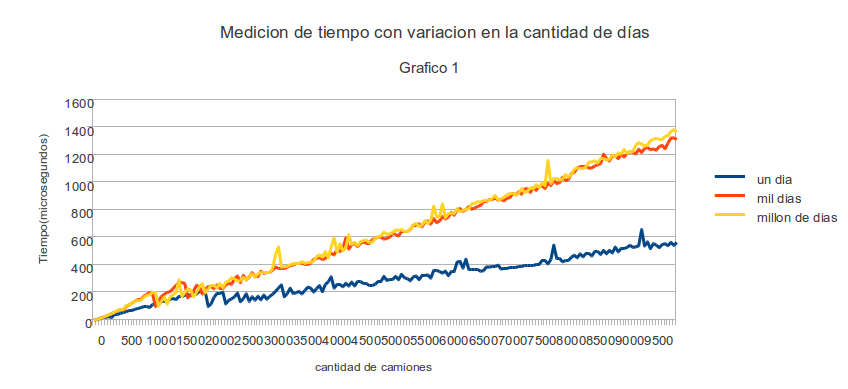
\includegraphics[width=1\textwidth]{grafico1-1}
  \label{fig:ejemplo}
\end{figure}


\paragraph{Gr�fico 2} Para este gr�fico usamos un intervalo de tama�o 1000000.

\begin{figure}[H]
    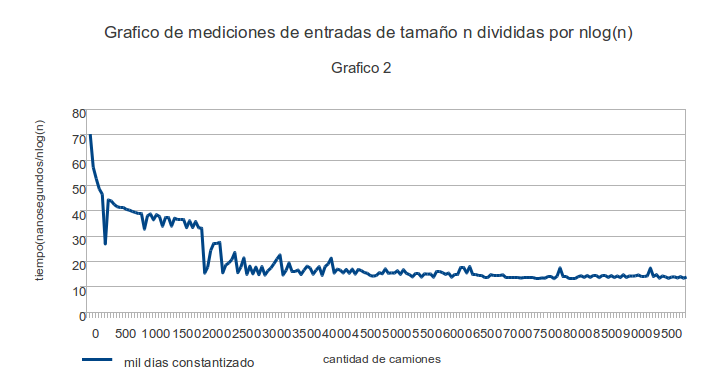
\includegraphics[width=1\textwidth]{grafico1-2}
  \label{fig:ejemplo}
\end{figure}

\subsubsection{Conclusiones} 
\paragraph{Gr�fico 1} En este gr�fico no solo queremos hacer notar que la complejidad asint�tica es de la pinta nLogn, sino que variar los
tama�os m�ximos de el par�metro de d�as m�ximos afecta a la complejidad del algoritmo.\\
\paragraph{Gr�fico 2} 
Lo que hacemos es $constantizar$ el gr�fico, es decir, dividimos las mediciones 
por la complejidad que calculamos, en este caso nLogn. Podemos notar que el gr�fico tiende a una constante. \\

\subsection{Desarrollo de los ejercicios adicionales}

\subsubsection{Modificaci�n al ejercicio}
Agregar la posibilidad de contratar al experto en dos periodos no necesariamente consecutivos de tiempo trae un problema interesante, pues ahora hay que tener en cuenta todos los posibles valores de K entre 1 y D, D siendo la cantidad de d�as total a contratar al experto, y K siendo la cantidad de d�as del primer periodo.\\

Notese que como K divide en dos periodos de contrato, desde ahora D1 y D2, podr�amos considerar que como un contrato de D d�as se divide en D1 = K y D2 = D-K esto seria lo mismo que D1 = D-K y D2 = K. En el cambio del algoritmo que propondremos D1 siempre estar� antes que D2, as� que como sabemos que en alg�n momento veremos que D2 esta antes que D1 por la propiedad arriba mencionada entonces no estamos perdiendo casos validos.\\

El cambio al algoritmo sera el siguiente, para cada k, correremos el algoritmo original con k como contrato, esto nos dar� el primer periodo �ptimo para k d�as de contrato por como funciona el algoritmo original, guardamos todos los datos y corremos nuevamente el algoritmo con el D-k, pero solamente le pasamos los camiones que llegan despu�s de que se termino el primer contrato y guardamos todos los datos en otras variables. sumo la cantidad de camiones que logre conseguir en ambos casos (si no quedan camiones en el segundo caso entonces sumo 0 y pongo el d�a de inicio de contrato justo despu�s de que termina el otro). ahora si podemos comparar el m�ximo conseguido con k hasta ahora con el m�ximo global y si es mayor guardar los datos. esto nos dara el maximo encontrado de correr el algoritmo con cada k.

\subsubsection{Complejidad y Conclusiones}
La nueva complejidad sera $O$($D*nlog(n)$) donde D es la longitud del contrato y n es la cantidad de camiones que llegaran. esto es as� pues hay que recorrer todos los k posibles entre 1 y D y correr el algoritmo original dos veces, y el algoritmo original era $O$($nlog(n)$), as� que ahora el algoritmo ya no depende solo de la cantidad de camiones que llegan, como era el caso original, sino que tambi�n depende de el tiempo del contrato.


\section{Problema 2: La joya del R�o de la Plata}

\subsection{Descripci�n del problema}
El problema consiste, en dada una lista de joyas, representadas por:\\
-un numero i entre 1 y n, con n la cantidad de joyas,que indica que la joya i fue la la iesima joya ingresada,\\
-un descuento por d�a de espera, y\\
-un tiempo de producci�n de cada joya,\\
devolver un orden, una lista sin repetidos con los n�meros de 1 a n, para fabricar las joyas, que minimice los descuentos 
generados por la demora en su fabricaci�n, junto con la perdida total de dinero.

Abstray�ndonos del contexto, este problema consiste en dad una secuencia $\Pi$ de n pares $(d,t)$ de n�meros positivos, devolver una lista X 
de n enteros entre 1 y n, sin repetidos, que representan cada uno la posici�n del par (joya) en la secuencia original $\Pi$ en un orden que 
minimice $ \sum_{i=1}^{n}(d_{i}( \sum_{j=1}^{i}t_{j})) $, junto con el valor de la misma.

Esta proviene del hecho de querer minimizar el descuento total, que se obtiene de la suma de los descuentos individuales, que a su vez se 
obtienen 
del descuento asociado a cada $joya_i$ ($d_i$) por el tiempo pasado hasta la entrega del mismo, es decir, su tiempo de fabricaci�n mas el 
de todas 
las joyas fabricadas previamente ($ \sum_{j=1}^{i}t_{j}$).
\\ 

\subsubsection{Ejemplos}
Sea X la lista de prioridad y D el descuento $\Rightarrow$
\begin{enumerate}
\item Par: (5,16) \\
La respuesta es �nica y es: X==[1] D==80.
\item Pares: (10,17)(1,9)\\
Las posibles respuestas son: 

\begin{center}
  
   \begin{tabular}{| l | c | r | }
     \hline
     Orden de prioridad & Descuento total \\ \hline
     [1,2] & 196 \\ \hline
     [2,1] & 277 \\ 
     \hline
   \end{tabular}
 \end{center}
Como 196 es menor, D==196 y X==[1,2].
\item Pares: (10,17) (20,20) (13,2) \\
Las posibles respuestas son: 

\begin{center}
  
   \begin{tabular}{| l | c | r | }
     \hline
     Orden de prioridad & Descuento total \\ \hline
     [1,2,3] & 1417 \\ \hline
     [1,3,2] & 1197 \\ \hline
     [2,1,3] & 1277 \\ \hline
     [2,3,1] & 1076 \\ \hline
     [3,1,2] & 996 \\ \hline
     [3,2,1] & 856 \\ 
     \hline
   \end{tabular}
 \end{center}
 
 Como 856 es menor, D==856 y X==[3,2,1]

\end{enumerate}

\subsection{Resoluci�n}

Para la resoluci�n de este problema optamos por realizar varios ejemplos, que no adjuntamos por ser demasiado tediosos, antes de plantear una 
soluci�n. En medio de esto, notamos un patr�n en cual mostraba que si la lista es una soluci�n �ptima, entonces esta ordenada de mayor a menor  
seg�n el cociente descuento-tiempo (d/t). 

Explorando esta posibilidad y la relaci�n entre los cocientes, llegamos al Lema 1, demostrado mas abajo, que dice que si
$\frac{\Pi_{d_{i}}}{\Pi_{t_{i}}} \leq \frac{\Pi_{d_{i+1}}}{\Pi_{t_{i+1}}}$
$\Rightarrow$ puedo permutar $\Pi_i$ y $\Pi_{i+1}$ obteniendo as� un descuento total menor.

Entonces la resoluci�n de este problema se basa en un algoritmo goloso. En cada momento, elegimos el elemento con mayor cociente 
descuento-tiempo (d/t) 
sin procesar.
Luego, una soluci�n �ptima proviene de ordenar la lista de manera decreciente de acuerdo al cociente descuento-tiempo. 

\subsubsection{Pseudoc�digo}
Aclaraci�n: la lista joyas aqu� mencionada, se pasa siempre por referencia.

\begin{algoritmo}{resolver}{\In{cantidadDeJoyas}{Nat}, \In{joyas}{Lista(Joya)}}[Lista(Joya)]
	Nat i \asignar 1\;
	\While{i $\leq$ cantidadDeJoyas}{
		calcular d/t\;
	}
	ordenar joyas de manera decreciente seg�n d/t\;
	calcular $\sum_{i=1}^{cantidadDeJoyas}(joyas_{d_{i}}( \sum_{j=1}^{i}joyas_{t_{j}}))$\;
	devolver joyas\;
\end{algoritmo}

\subsection{Correctitud}
\subsubsection{Idea}
Sea $\Pi$ una permutaci�n �ptima de $\Omega$, con $\Omega$ la lista de joyas original, quiero demostrar que existe $\Pi'$ ordenada de manera 
decreciente seg�n
cociente descuento-tiempo, que tambi�n es �ptima. Para esto, basta ver que si tengo dos elementos
$\Pi_i$ y $\Pi_{i+1}$, tales que $\frac{\Pi_{d_{i}}}{\Pi_{t_{i}}} \leq \frac{\Pi_{d_{i+1}}}{\Pi_{t_{i+1}}} $, puedo permutarlos
obteniendo as� un resultado menor, o igual, para la sumatoria. 

Luego, ordenando la sumatoria con este criterio, mediante alg�n algoritmo similar a 
bubble sort, obtengo una permutaci�n $\Pi'$, a partir de $\Pi$, que 
est� ordenada y da un resultado igual, pues no puede ser mejor ya que asumimos $\Pi$ �ptima, 
al de la soluci�n �ptima. 

Para finalizar, definiremos un orden determin�stico, para asegurarnos as� que solo existe una
permutaci�n de $\Pi$ que est� ordenada. Con esto quedar�a demostrado que $\Pi'$ es una soluci�n �ptima.
\\

\subsubsection{Lema 1: Intercambio de $\Pi$'s}
\textbf{ Si $\frac{\Pi_{d_{i}}}{\Pi_{t_{i}}} \leq \frac{\Pi_{d_{i+1}}}{\Pi_{t_{i+1}}}$
$\Rightarrow$ puedo permutar $\Pi_i$ y $\Pi_{i+1}$ obteniendo as� un descuento total menor.}

-Queremos ver que podemos permutar $\Pi_i$ y $\Pi_{i+1}$:\\
S� que si  $\Pi_i$ y $\Pi_{i+1}$ tienen la siguiente propiedad\\
$\frac{\Pi_{d_{i}}}{\Pi_{t_{i}}} \leq \frac{\Pi_{d_{i+1}}}{\Pi_{t_{i+1}}} \Rightarrow $ 
$ \Pi_{d_{i}}\Pi_{t_{i+1}} \leq\Pi_{d_{i+1}}\Pi_{t_{i}} \Rightarrow$ 
$0 \leq  \Pi_{d_{i+1}}\Pi_{t_{i}}- \Pi_{d_{i}}\Pi_{t_{i+1}}$\\
Ahora queremos ver las sumatorias de $\Pi$ y $\Pi'$\\
$SUM(\Pi)=\sum_{j=1}^{n}(\Pi_{d_{j}}( \sum_{k=1}^{j}\Pi_{t_{k}}))$\\
$SUM(\Pi')= \sum_{j=1}^{i-1}(\Pi_{d_{j}}( \sum_{k=1}^{j}\Pi_{t_{k}}))
+ \Pi_{d_{i+1}}( \sum_{k=1}^{i-1}\Pi_{t_{k}}+ \Pi_{t_{i+1}})
+ \Pi_{d_{i}}( \sum_{k=1}^{i+1}\Pi_{t_{k}})
+ \sum_{j=i+2}^{n}(\Pi_{d_{j}}( \sum_{k=1}^{j}\Pi_{t_{k}}))
$\\

N�tese que la sumatoria de $\Pi'$ esta escrita en base a la permutaci�n $\Pi$. Esto es para poder realizar cuentas 
entre ambas sumatorias, porque de otro modo deber�amos probar que los t�rminos sean iguales por separado, lo que nos
restar�a claridad.\\

Luego $SUM(\Pi)-SUM(\Pi') = \\
\sum_{j=1}^{n}(\Pi_{d_{j}}(\sum_{k=1}^{j}(\Pi_{t_{k}}))) -
\sum_{j=1}^{i-1}(\Pi_{d_{j}}(\sum_{k=1}^{j}(\Pi_{t_{k}}))) -
\Pi_{d_{i+1}}(\sum_{k=1}^{i-1}(\Pi_{t_{k}})+\Pi_{t_{i+1}}) -
\Pi_{d_{i}}(\sum_{k=1}^{i+1}(\Pi_{t_{k}}))-
\sum_{j=i+2}^{n}(\Pi_{d_{j}}(\sum_{k=1}^{j}(\Pi_{t_{k}}))) = \\ \\
\xcancel{\sum_{j=i-1}^{n}(\Pi_{d_{j}}(\sum_{k=1}^{j}(\Pi_{t_{k}})))} +
\Pi_{d_{i}}(\sum_{k=1}^{i}(\Pi_{t_{k}})) +
\Pi_{d_{i+1}}(\sum_{k=1}^{i+1}(\Pi_{t_{k}}))+
\xcancel{\sum_{j=i+2}^{n}(\Pi_{d_{j}}(\sum_{k=1}^{j}(\Pi_{t_{k}})))}-
\xcancel{\sum_{j=1}^{i-1}(\Pi_{d_{j}}(\sum_{k=1}^{j}(\Pi_{t_{k}})))} -
\Pi_{d_{i+1}}(\sum_{k=1}^{i-1}(\Pi_{t_{k}})+\Pi_{t_{i+1}}) -
\Pi_{d_{i}}(\sum_{k=1}^{i+1}(\Pi_{t_{k}}))-
\xcancel{\sum_{j=i+2}^{n}(\Pi_{d_{j}}(\sum_{k=1}^{j}(\Pi_{t_{k}})))} = \\ \\ 
\Pi_{d_{i}}(\sum_{k=1}^{i}(\Pi_{t_{k}})) +
\Pi_{d_{i+1}}(\sum_{k=1}^{i+1}(\Pi_{t_{k}}))-
\Pi_{d_{i+1}}(\sum_{k=1}^{i-1}(\Pi_{t_{k}})+\Pi_{t_{i+1}}) -
\Pi_{d_{i}}(\sum_{k=1}^{i+1}(\Pi_{t_{k}})) = \\ \\
\xcancel{\Pi_{d_{i}}(\sum_{k=1}^{i}(\Pi_{t_{k}}))} +
\xcancel{\Pi_{d_{i+1}}(\sum_{k=1}^{i-1}(\Pi_{t_{k}}))}+
\Pi_{d_{i+1}}\Pi_{t_{i}}+
\xcancel{\Pi_{d_{i+1}}\Pi_{t_{i+1}}}-
\xcancel{\Pi_{d_{i+1}}(\sum_{k=1}^{i-1}(\Pi_{t_{k}}))} -
\xcancel{\Pi_{d_{i+1}}\Pi_{t_{i+1}}}-
\xcancel{\Pi_{d_{i}}(\sum_{k=1}^{i}(\Pi_{t_{k}}))}-
\Pi_{d_{i}}\Pi_{t_{i+1}}=\\ \\
\Pi_{d_{i+1}}\Pi_{t_{i}}-
\Pi_{d_{i}}\Pi_{t_{i+1}}\geq 0.
$
(por propiedad de $\Pi_i $ y $ \Pi_{i+1}$) \\

Luego $SUM(\Pi)-SUM(\Pi')\geq0$
por lo tanto $SUM(\Pi) \geq SUM(\Pi')$, lo que nos asegura que si permutamos los elementos, obtenemos una soluci�n mejor o igual.

\subsubsection{Lema 2: Definici�n de un orden determin�stico}
\textbf{Hay una �nica secuencia ordenada.}

Sea $\Pi_i$, $\Pi_{i+1}$ tales que 
$\frac{\Pi_{d_{i}}}{\Pi_{t_{i}}} < \frac{\Pi_{d_{i+1}}}{\Pi_{t_{i+1}}} $
, defino que el orden como $\Pi_{i+1}$ predecesor de $\Pi_{i}$. Si estoy en el caso 
$\frac{\Pi_{d_{i}}}{\Pi_{t_{i}}} = \frac{\Pi_{d_{i+1}}}{\Pi_{t_{i+1}}} $
defino como predecesor a aquel que tenga mayor d. Si estoy en el caso 
$\frac{\Pi_{d_{i}}}{\Pi_{t_{i}}} > \frac{\Pi_{d_{i+1}}}{\Pi_{t_{i+1}}} $ defino a $\Pi_{i}$ predecesor de $\Pi_{i+1}$. 
N�tese, que si $\Pi_{i+1}$ es igual a $\Pi_{i}$, entonces el ninguno es el predecesor, pues son el mismo elemento. Luego 
permutarlos o no hacerlo nos devuelve la misma lista.

\subsubsection{Conclusi�n}
Ahora sabemos que dada cualquier secuencia $\Pi$ podemos ordenarla y vamos a conseguir un descuento menor o igual al de la original, por lema 1,
y tambi�n sabemos que solo hay una secuencia $\Pi'$ ordenada, por lema 2, es decir que $\forall \Pi, SUM(\Pi)\leq SUM(\Pi')$, luego $\Pi'$ 
es �ptima.


\subsection{Complejidad}
\subsubsection{Introducci�n}
Puede comprobarse en el c�digo que, omitiendo la carga de datos y las iteraciones requeridas
para manejar las distintas instancias del problema, el algoritmo ejecutado para la resoluci�n del problema es el siguiente.

Debajo del algoritmo se encuentran varias aclaraciones identificadas por el n�mero de l�nea.

Sea n la cantidad de elementos de la lista, Joya un tipo tupla con tres elementos (Nat n, double d, double t).
\subsubsection{Pseudoc�digo}
\begin{algoritmo}{resolver}{\In{joyas}{Lista(Joya)}}
\LinesNumbered
\nl	joyas.sort(criterioDeComparacion)\tcc*{$O$(nLogn)}
	Nat montoPerdido \asignar 0\tcc*{$O$(1)}
	Nat diasTranscurridos \asignar 0\tcc*{$O$(1)}
	\For(\tcc*[f]{$O$($n$)}){(it \asignar joyas.begin(); it != joyas.end(); it++)}{
		double d, t\tcc*{$O$(1)}
		Joya npieza \asignar *it\tcc*{$O$(1)}
		d \asignar npieza.d\tcc*{$O$(1)}
		diasTranscurridos \asignar diasTranscurridos + t\tcc*{$O$(1)}
		montoPerdido \asignar montoPerdido + diasTranscurridos*d\tcc*{$O$(1)}
	}
	\return joyas \tcc*{$O$(1)}
	\return montoPerdido \tcc*{$O$(1)}
\end{algoritmo}

\begin{algoritmo}{criterioDeComparacion}{\In{joya1}{Joya}, \In{joya2}{Joya}}[bool]
\LinesNumbered
\setcounter{AlgoLine}{12}
\nl	double d1, t1, d2, t2\tcc*{$O$(1)}
	d1 \asignar joya1.d\tcc*{$O$(1)}
	t1 \asignar joya1.t\tcc*{$O$(1)}
	d2 \asignar joya2.d\tcc*{$O$(1)}
	t2 \asignar joya2.t\tcc*{$O$(1)}
	\uIf(\tcc*[f]{$O$(1)}){ (d1/t1 $\neq$ d2/t2)}{
		\return ( d1/t1 $>$ d2/t2 )\tcc*{$O$(1)}
	}
	\Else{
		\return ( d1 $>$ d2 )\tcc*{$O$(1)}
	}
\end{algoritmo} 

\subsubsection{Aclaraciones del Pseudoc�digo} 
1) V�ase en http://en.cppreference.com/w/cpp/container/list/sort, la complejidad es $nlogn$ comparaciones, pero
como, por l�nea 13) y siguientes, las comparaciones son $O$(1), la complejidad final es $O$($nlogn$).\\
6) Crear un iterador, avanzarlo, y compararlo es O(1), y todas las llamadas internas del for son O(1), luego, la complejidad
del mismo son la cantidad de iteraciones necesarias para finalizarlo, en este caso, n. Luego, la complejidad del for es O(n).\\
11) Si bien retornar una lista de n elementos no es O(1), en este contexto, y como lo pasamos por referencia, no nos interesa 
considerar la complejidad que tomar�a mostrarla en pantalla. \\
11 y 12) Esto es un abuso de lenguaje, as� que aclaramos que la funci�n no devuelve dos cosas distintas sino que devuelve 
ambas cosas en una sola instancia. O, si lo leemos desde el c�digo fuente, modifica joyas y devuelve solo el monto perdido, pero 
escribirlo de esa manera en el pseudo cogido restar�a claridad y no aportar�a nada muy importante, ya que es un detalle 
m�nimo de implementaci�n que no modifica la complejidad.

\subsubsection{Conclusi�n}

Como este algoritmo es iterativo, o sea no tiene partes recursivas, la complejidad total es la suma de las complejidades, luego si sumamos 
las complejidades de cada linea obtenemos que este algoritmo es O(nLogn), siendo n la cantidad de joyas a ordenar.

\subsection{Testing}
Los casos bordes que consideramos en este ejercicio son los que tienen los mismos elementos pero permutados, aquellos que 
tienen la misma proporci�n entre d y t, y los que tienen un solo elemento. Para ello, usamos las siguientes entradas.
\begin{center}
  \begin{tabular}{| l | c | r | c | r |c | r | }
    \hline
     Cantidad de Joyas & Joyas & Orden de prioridad & Descuento \\ \hline
     1 & [(1,1)] & [1] & 1 \\ \hline
     1 & [(1,5)] & [1] & 5 \\ \hline
     1 & [(3,2)] & [1] & 6 \\ \hline
     5 & [(1,2),(2,4),(3,6),(8,16),(10,20)] & [5,4,3,2,1] & 754 \\ \hline
     5 & [(10,20),(8,16),(3,6),(2,4),(1,2)] & [1,2,3,4,5] & 754 \\ \hline
     3 & [(1,4),(1,4),(4,16)] & [3,1,2] & 108 \\ \hline
     3 & [(1,4),(4,16),(1,4)] & [2,1,3] & 108 \\ 
     \hline
   \end{tabular}
 \end{center}
\paragraph{Nota}
La validez de estos resultados se comprob� a mano, mas no se adjuntan las cuentas pues creemos que no aportan mucho mas que espacio
malgastado. (Salvemos un �rbol! Ahorremos papel!)

\subsection{Experimentaci�n}
Para la experimentaci�n, generamos instancias aleatorias de distintos tama�os, variando el tope m�ximo d y t. Siendo n el tama�o 
la entrada. L�ase por aleatoria, creada por la funci�n Rand() de C++ y manipulada lo m�nimamente necesario para que diera un numero razonable.
La manipulaci�n se muestra en el Anexo del c�digo, en la parte correspondiente al archivo $ejemplos\_random.cpp$.

\paragraph{Gr�fico 3}
Para este gr�fico usamos los topes 100 y 1000, adem�s se contempla el caso en el que el coeficiente de todas las joyas de siempre igual,
muestra el tiempo, en nanosegundos, requerido para resolver el problema.

\paragraph{Gr�fico 4}
Para este gr�fico usamos el tope 1000. Lo que hacemos es $constantizar$ el gr�fico, es decir, dividimos las mediciones 
por la complejidad que calculamos, en este caso nLogn. \\

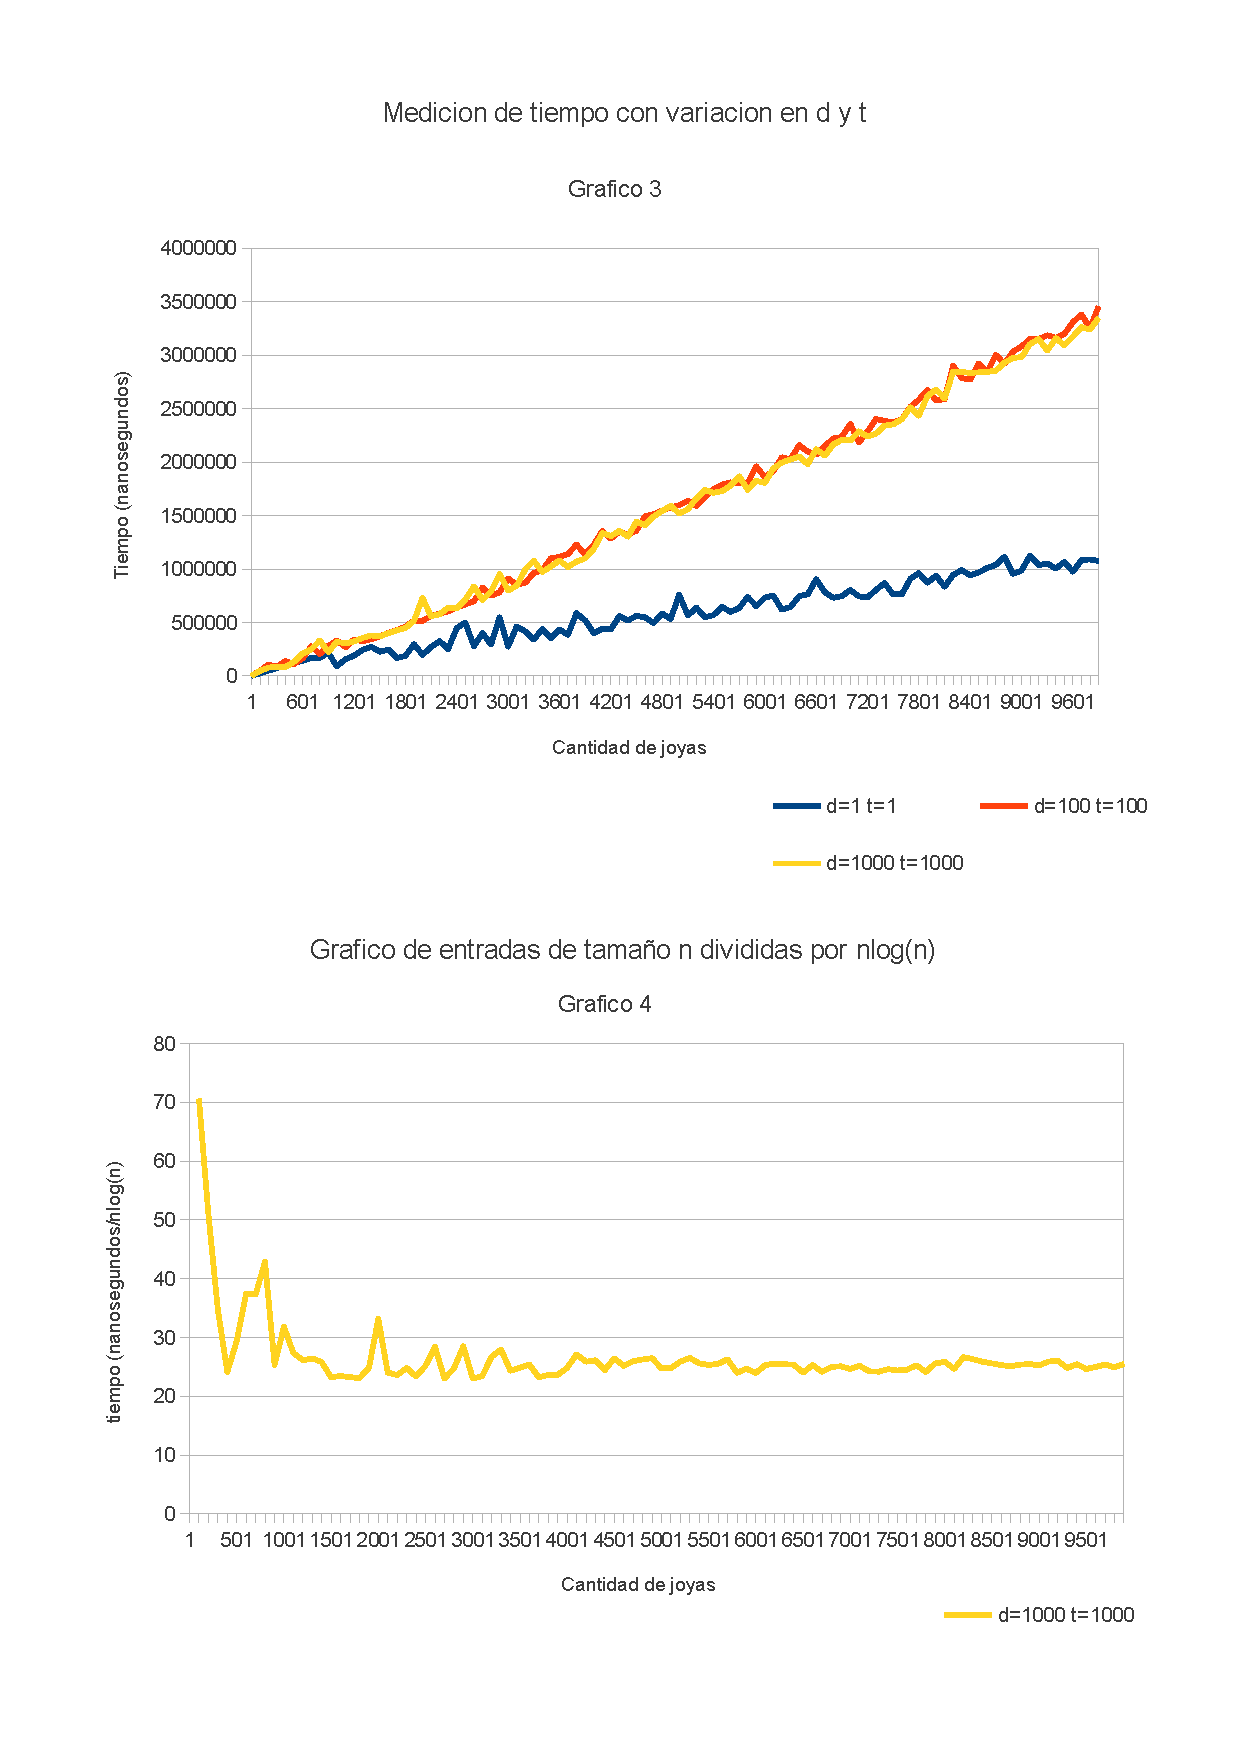
\includepdf[pages={1}]{grafp2.pdf}
\subsubsection{Conclusiones} 
\paragraph{Gr�fico 3}
En este gr�fico el caso base extremo, denotado con la linea azul, muestra que si todas las joyas tienen el mismo coeficiente, dar el orden es 
mucho mas f�cil.
Luego podemos ver que no hay casi variaci�n en el costo de ordenarlas si son distintas, aun cuando varia el valor m�ximo de los costos. Esto
nos muestra que en realidad el tiempo de resoluci�n no depende tanto de los valores d y t de cada joya, sino que depende en mayor medida de la
variaci�n entre coeficientes.

\paragraph{Gr�fico 4}
Queremos hacer notar que el gr�fico tiende a una constante, es decir, que efectivamente la complejidad es la esperada. \\

\subsection{Desarrollo de los ejercicios adicionales}

\subsubsection{Modificaci�n al ejercicio}

Para la resolver este nuevo problema mantenemos b�sicamente el mismo algoritmo, porque todas las ideas mencionadas previamente siguen
valiendo. La �nica modificaci�n grande, enti�ndase por "peque�as" aquellas
como cambiar el tipo joya a una tupla de tres elementos y similares, se hace en el criterio de orden, que cambiaremos por el descripto 
a continuaci�n.

\begin{algoritmo}{criterioDeComparacion}{\In{joya1}{Joya}, \In{joya2}{Joya}}[bool]
\LinesNumbered
\setcounter{AlgoLine}{12}
\nl	double d1, t1, r1, d2, t2, r2\tcc*{$O$(1)}
	d1 \asignar joya1.d\tcc*{$O$(1)}
	t1 \asignar joya1.t\tcc*{$O$(1)}
	r1 \asignar joya1.r\tcc*{$O$(1)}
	d2 \asignar joya2.d\tcc*{$O$(1)}
	t2 \asignar joya2.t\tcc*{$O$(1)}
	r2 \asignar joya2.r\tcc*{$O$(1)}
	\uIf(\tcc*[f]{$O$(1)}){ (d1/(t1+r1) $\neq$ d2/(t2+r1))}{
		\return ( d1/t1 $>$ d2/t2 )\tcc*{$O$(1)}
	}
	\Else{
		\uIf(\tcc*[f]{$O$(1)}){ d1 $\neq$ d2}{
		    \return ( d1 $>$ d2 )\tcc*{$O$(1)}
		}
		\Else{
		    \return ( r1 $>$ r2 )\tcc*{$O$(1)}
	      }
	}
\end{algoritmo} 

En todo lo dem�s, el algoritmo es el mismo que en el ejercicio original.

\subsubsection{Demostraci�n}

Como primera medida, n�tese que el algoritmo es casi igual al original, por lo que tanto la idea de la demostraci�n como
su conclusi�n, son id�nticas. Lo �nico que necesitamos modificar son los lemas, de tal
manera que contemplen el nuevo par�metro.

\subsubsection{Lema 1'}
\textbf{ Si $\frac{\Pi_{d_{i}}}{(\Pi_{t_{i}}+\Pi_{r_{i}})} \leq \frac{\Pi_{d_{i+1}}}{(\Pi_{t_{i+1}}+\Pi_{r_{i+1}})}$
$\Rightarrow$ puedo permutar $\Pi_i$ y $\Pi_{i+1}$ obteniendo as� un descuento total menor.}

-Queremos ver que podemos permutar $\Pi_i$ y $\Pi_{i+1}$:\\
S� que si  $\Pi_i$ y $\Pi_{i+1}$ tienen la siguiente propiedad\\
$\frac{\Pi_{d_{i}}}{(\Pi_{t_{i}}+\Pi_{r_{i}})} \leq \frac{\Pi_{d_{i+1}}}{(\Pi_{t_{i+1}}+\Pi_{r_{i+1}})} \Rightarrow $ 
$ \Pi_{d_{i}}(\Pi_{t_{i+1}}+\Pi_{r_{i+1}}) \leq\Pi_{d_{i+1}}(\Pi_{t_{i}}+\Pi_{r_{i}}) \Rightarrow$ 
$0 \leq  \Pi_{d_{i+1}}(\Pi_{t_{i}}+\Pi_{r_{i}})- \Pi_{d_{i}}(\Pi_{t_{i+1}}+\Pi_{r_{i+1}})$\\

Ahora queremos ver las sumatorias de $\Pi$ y $\Pi'$\\
$SUM(\Pi)=\sum_{j=1}^{n}(\Pi_{d_{j}}( \sum_{k=1}^{j}\Pi_{t_{k}} + \sum_{h=1}^{j-1}\Pi_{r_{h}}))$\\
$SUM(\Pi')= \sum_{j=1}^{i-1}(\Pi_{d_{j}}( \sum_{k=1}^{j}\Pi_{t_{k}} + \sum_{h=1}^{j-1}\Pi_{r_{h}}))
+ \Pi_{d_{i+1}}( \sum_{k=1}^{i-1}\Pi_{t_{k}}+ \Pi_{t_{i+1}} + \sum_{h=1}^{i-1}\Pi_{r_{h}})
+ \Pi_{d_{i}}( \sum_{k=1}^{i-1}\Pi_{t_{k}} + \Pi_{t_{i+1}} + \Pi_{t_{i}} + \sum_{h=1}^{i-1}\Pi_{r_{h}} + \Pi_{r_{i+1}})
+ \sum_{j=i+2}^{n}(\Pi_{d_{j}}( \sum_{k=1}^{j}\Pi_{t_{k}} + \sum_{h=1}^{j-1}\Pi_{r_{h}}))
$\\

N�tese que la sumatoria de $\Pi'$ esta escrita en base a la permutaci�n $\Pi$. Esto es para poder realizar cuentas 
entre ambas sumatorias, porque de otro modo deber�amos probar que los t�rminos sean iguales por separado, lo que nos
restar�a claridad.\\

Luego $SUM(\Pi)-SUM(\Pi') = \\\sum_{j=1}^{n}(\Pi_{d_{j}}( \sum_{k=1}^{j}\Pi_{t_{k}} + \sum_{h=1}^{j-1}\Pi_{r_{h}})) -
\sum_{j=1}^{i-1}(\Pi_{d_{j}}( \sum_{k=1}^{j}\Pi_{t_{k}} + \sum_{h=1}^{j-1}\Pi_{r_{h}})) -
 \Pi_{d_{i+1}}( \sum_{k=1}^{i-1}\Pi_{t_{k}}+ \Pi_{t_{i+1}} + \sum_{h=1}^{i-1}\Pi_{r_{h}})-
 \Pi_{d_{i}}( \sum_{k=1}^{i-1}\Pi_{t_{k}} + \Pi_{t_{i+1}} + \Pi_{t_{i}} + \sum_{h=1}^{i-1}\Pi_{r_{h}} + \Pi_{r_{i+1}})-
 \sum_{j=i+2}^{n}(\Pi_{d_{j}}( \sum_{k=1}^{j}\Pi_{t_{k}} + \sum_{h=1}^{j-1}\Pi_{r_{h}})) = 
\\ \\
\xcancel{\sum_{j=1}^{i-1}(\Pi_{d_{j}}( \sum_{k=1}^{j}\Pi_{t_{k}} + \sum_{h=1}^{j-1}\Pi_{r_{h}}))} +
 \Pi_{d_{i}}( \xcancel{\sum_{k=1}^{i-1}\Pi_{t_{k}}}+ \xcancel{\Pi_{t_{i}}} + \xcancel{\sum_{h=1}^{i-1}\Pi_{r_{h}})}+
 \Pi_{d_{i+1}}( \xcancel{\sum_{k=1}^{i-1}\Pi_{t_{k}}} + \xcancel{\Pi_{t_{i+1}}} + \Pi_{t_{i}} +\xcancel{ \sum_{h=1}^{i-1}\Pi_{r_{h}}} + \Pi_{r_{i}})+
 \xcancel{\sum_{j=i+2}^{n}(\Pi_{d_{j}}( \sum_{k=1}^{j}\Pi_{t_{k}} + \sum_{h=1}^{j-1}\Pi_{r_{h}}))}-
\xcancel{\sum_{j=1}^{i-1}(\Pi_{d_{j}}( \sum_{k=1}^{j}\Pi_{t_{k}} + \sum_{h=1}^{j-1}\Pi_{r_{h}}))} -
 \Pi_{d_{i+1}}( \xcancel{\sum_{k=1}^{i-1}\Pi_{t_{k}}}+ \xcancel{\Pi_{t_{i+1}}} + \xcancel{\sum_{h=1}^{i-1}\Pi_{r_{h}}})-
 \Pi_{d_{i}}(\xcancel{ \sum_{k=1}^{i-1}\Pi_{t_{k}}} + \Pi_{t_{i+1}} + \xcancel{\Pi_{t_{i}}} + \xcancel{\sum_{h=1}^{i-1}\Pi_{r_{h}}} + \Pi_{r_{i+1}})-
 \xcancel{\sum_{j=i+2}^{n}(\Pi_{d_{j}}( \sum_{k=1}^{j}\Pi_{t_{k}} + \sum_{h=1}^{j-1}\Pi_{r_{h}}))} =
 \\ \\
 \Pi_{d_{i+1}}(\Pi_{t_{i}}+\Pi_{r_{i}})- \Pi_{d_{i}}(\Pi_{t_{i+1}}+\Pi_{r_{i+1}})\geq 0 $
(por propiedad de $\Pi_i $ y $ \Pi_{i+1}$) \\

Luego $SUM(\Pi)-SUM(\Pi')\geq0$
por lo tanto $SUM(\Pi) \geq SUM(\Pi')$, lo que nos asegura que si permutamos los elementos, obtenemos una soluci�n mejor o igual.

\paragraph{Lema 2'} Este lema que define que solo hay un orden, es extensible de manera trivial al par�metro. La forma es agregar en el 
caso de la igualdad, si estoy en el caso en el ambos tienen el par�metro d
igual, definir� como predecesor a aquel que tenga mayor r. El resto de la demostraci�n es igual.\\

En conclusi�n, con estos nuevos lemas, la demostraci�n es la misma que en el punto 3.3



\newpage
\section{Problema 3: Rompecolores}

\subsection{Descripci�n del problema}

El problema de los Rompecolores consiste en un tablero de $n$ filas y $m$ columnas, y una cantidad de piezas igual a $n*m$. Cada pieza tiene 4 lados, los cuales pueden tener un color entre $1$ y $c$. 
El objetivo es colocar las piezas en el tablero, de manera tal que, para cada pieza colocada, el color de cada uno de sus lados coincide con el color del lado adyacente de las piezas colocadas alrededor si las hubiera. Se debe buscar la soluci�n que m�s piezas tenga en el tablero.
%La entrada del problema consiste de una l�nea indicando las dimensiones del tablero (n y m) y la cantidad distinta de colores posibles (c). 
%A esta l�nea le siguen $n*m$ l�neas, cada una de las cuales consta de 4 enteros entre 1 y c, los cuales representan los colores de los lados superior, izquierdo, derecho e inferior, respectivamente.
%La salida del problema consiste de n l�neas, y en cada l�nea m n�meros, cada uno de estos n�meros representando el estado del tablero en la posici�n ($n_i$,$m_j$).
%Si ($n_i$,$m_j$) es 0, no se coloc� ninguna pieza en esa posici�n; en caso contrario, indica el n�mero de la pieza.

\subsubsection{Ejemplos}

\begin{figure}[H]
    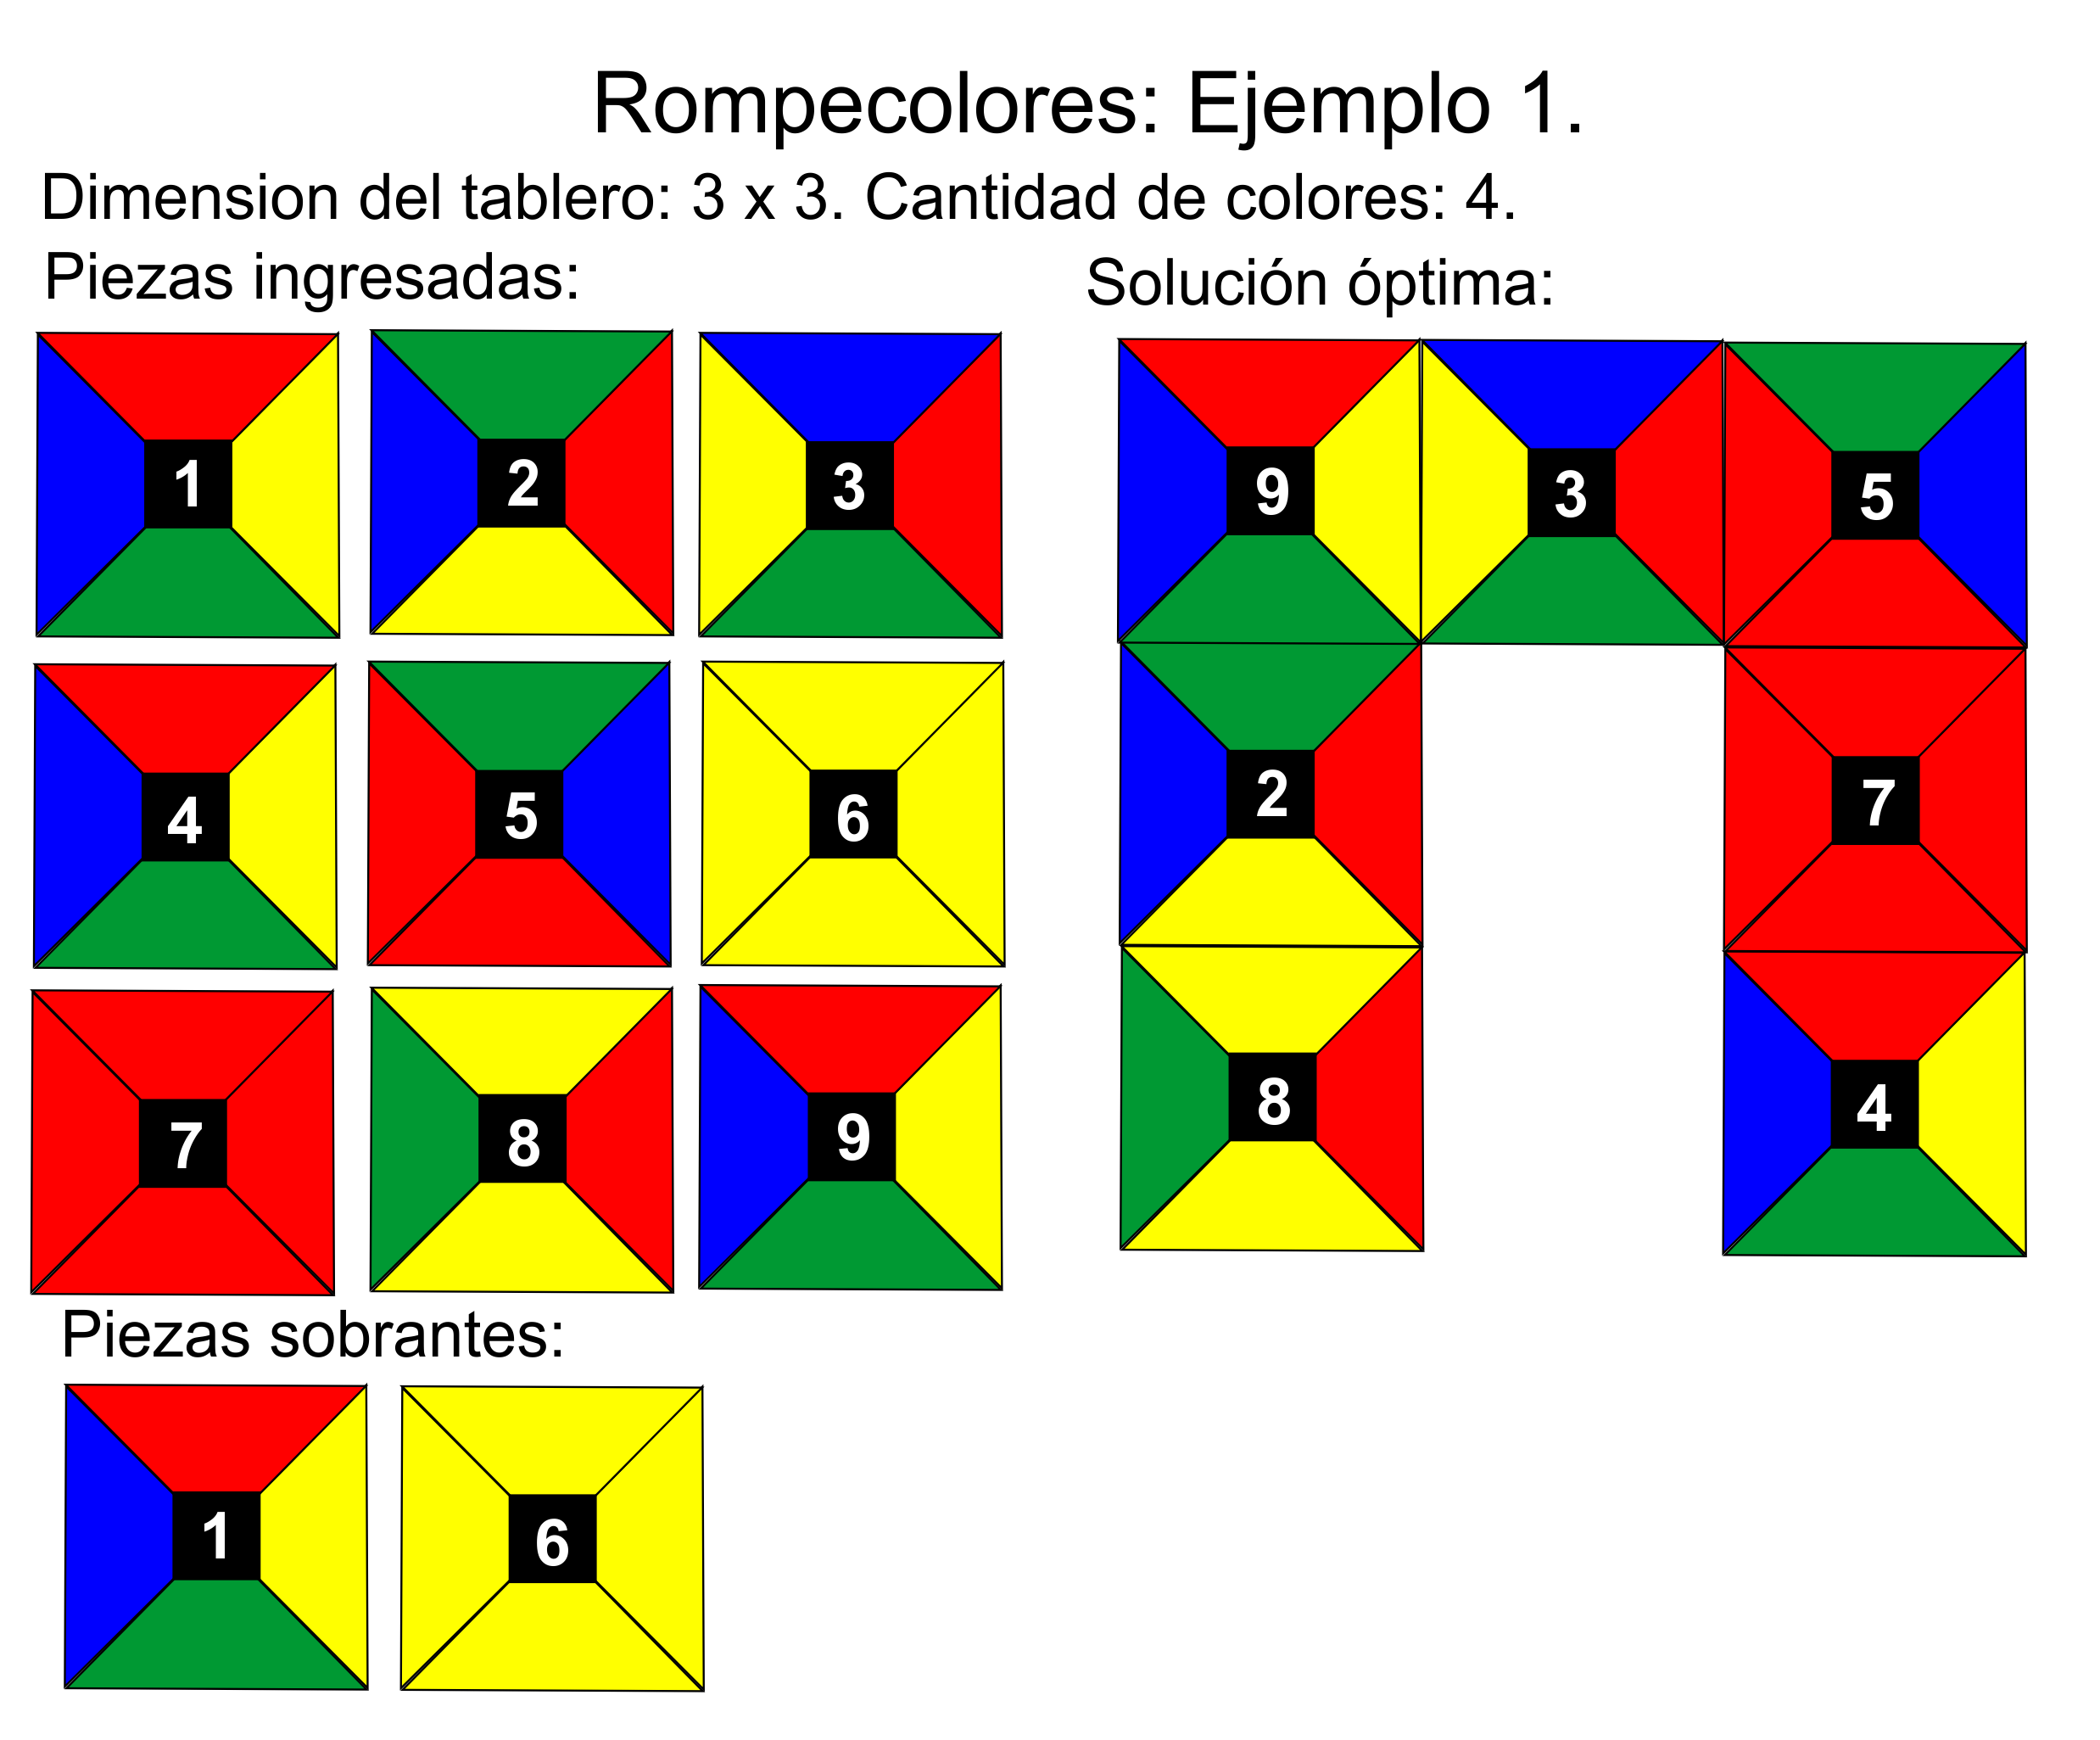
\includegraphics[width=0.6\textwidth]{ejemplo1Compacto}
  \label{fig:ejemplo}
  \caption{Esta es una soluci�n �ptima porque no hay otro orden donde podamos a�adir m�s de 7 piezas. Fue calculada con el algoritmo sin podas.}
\end{figure}


Esta soluci�n fue obtenida con el algoritmo de backtracking 2 sin podas.

\begin{figure}[H]
    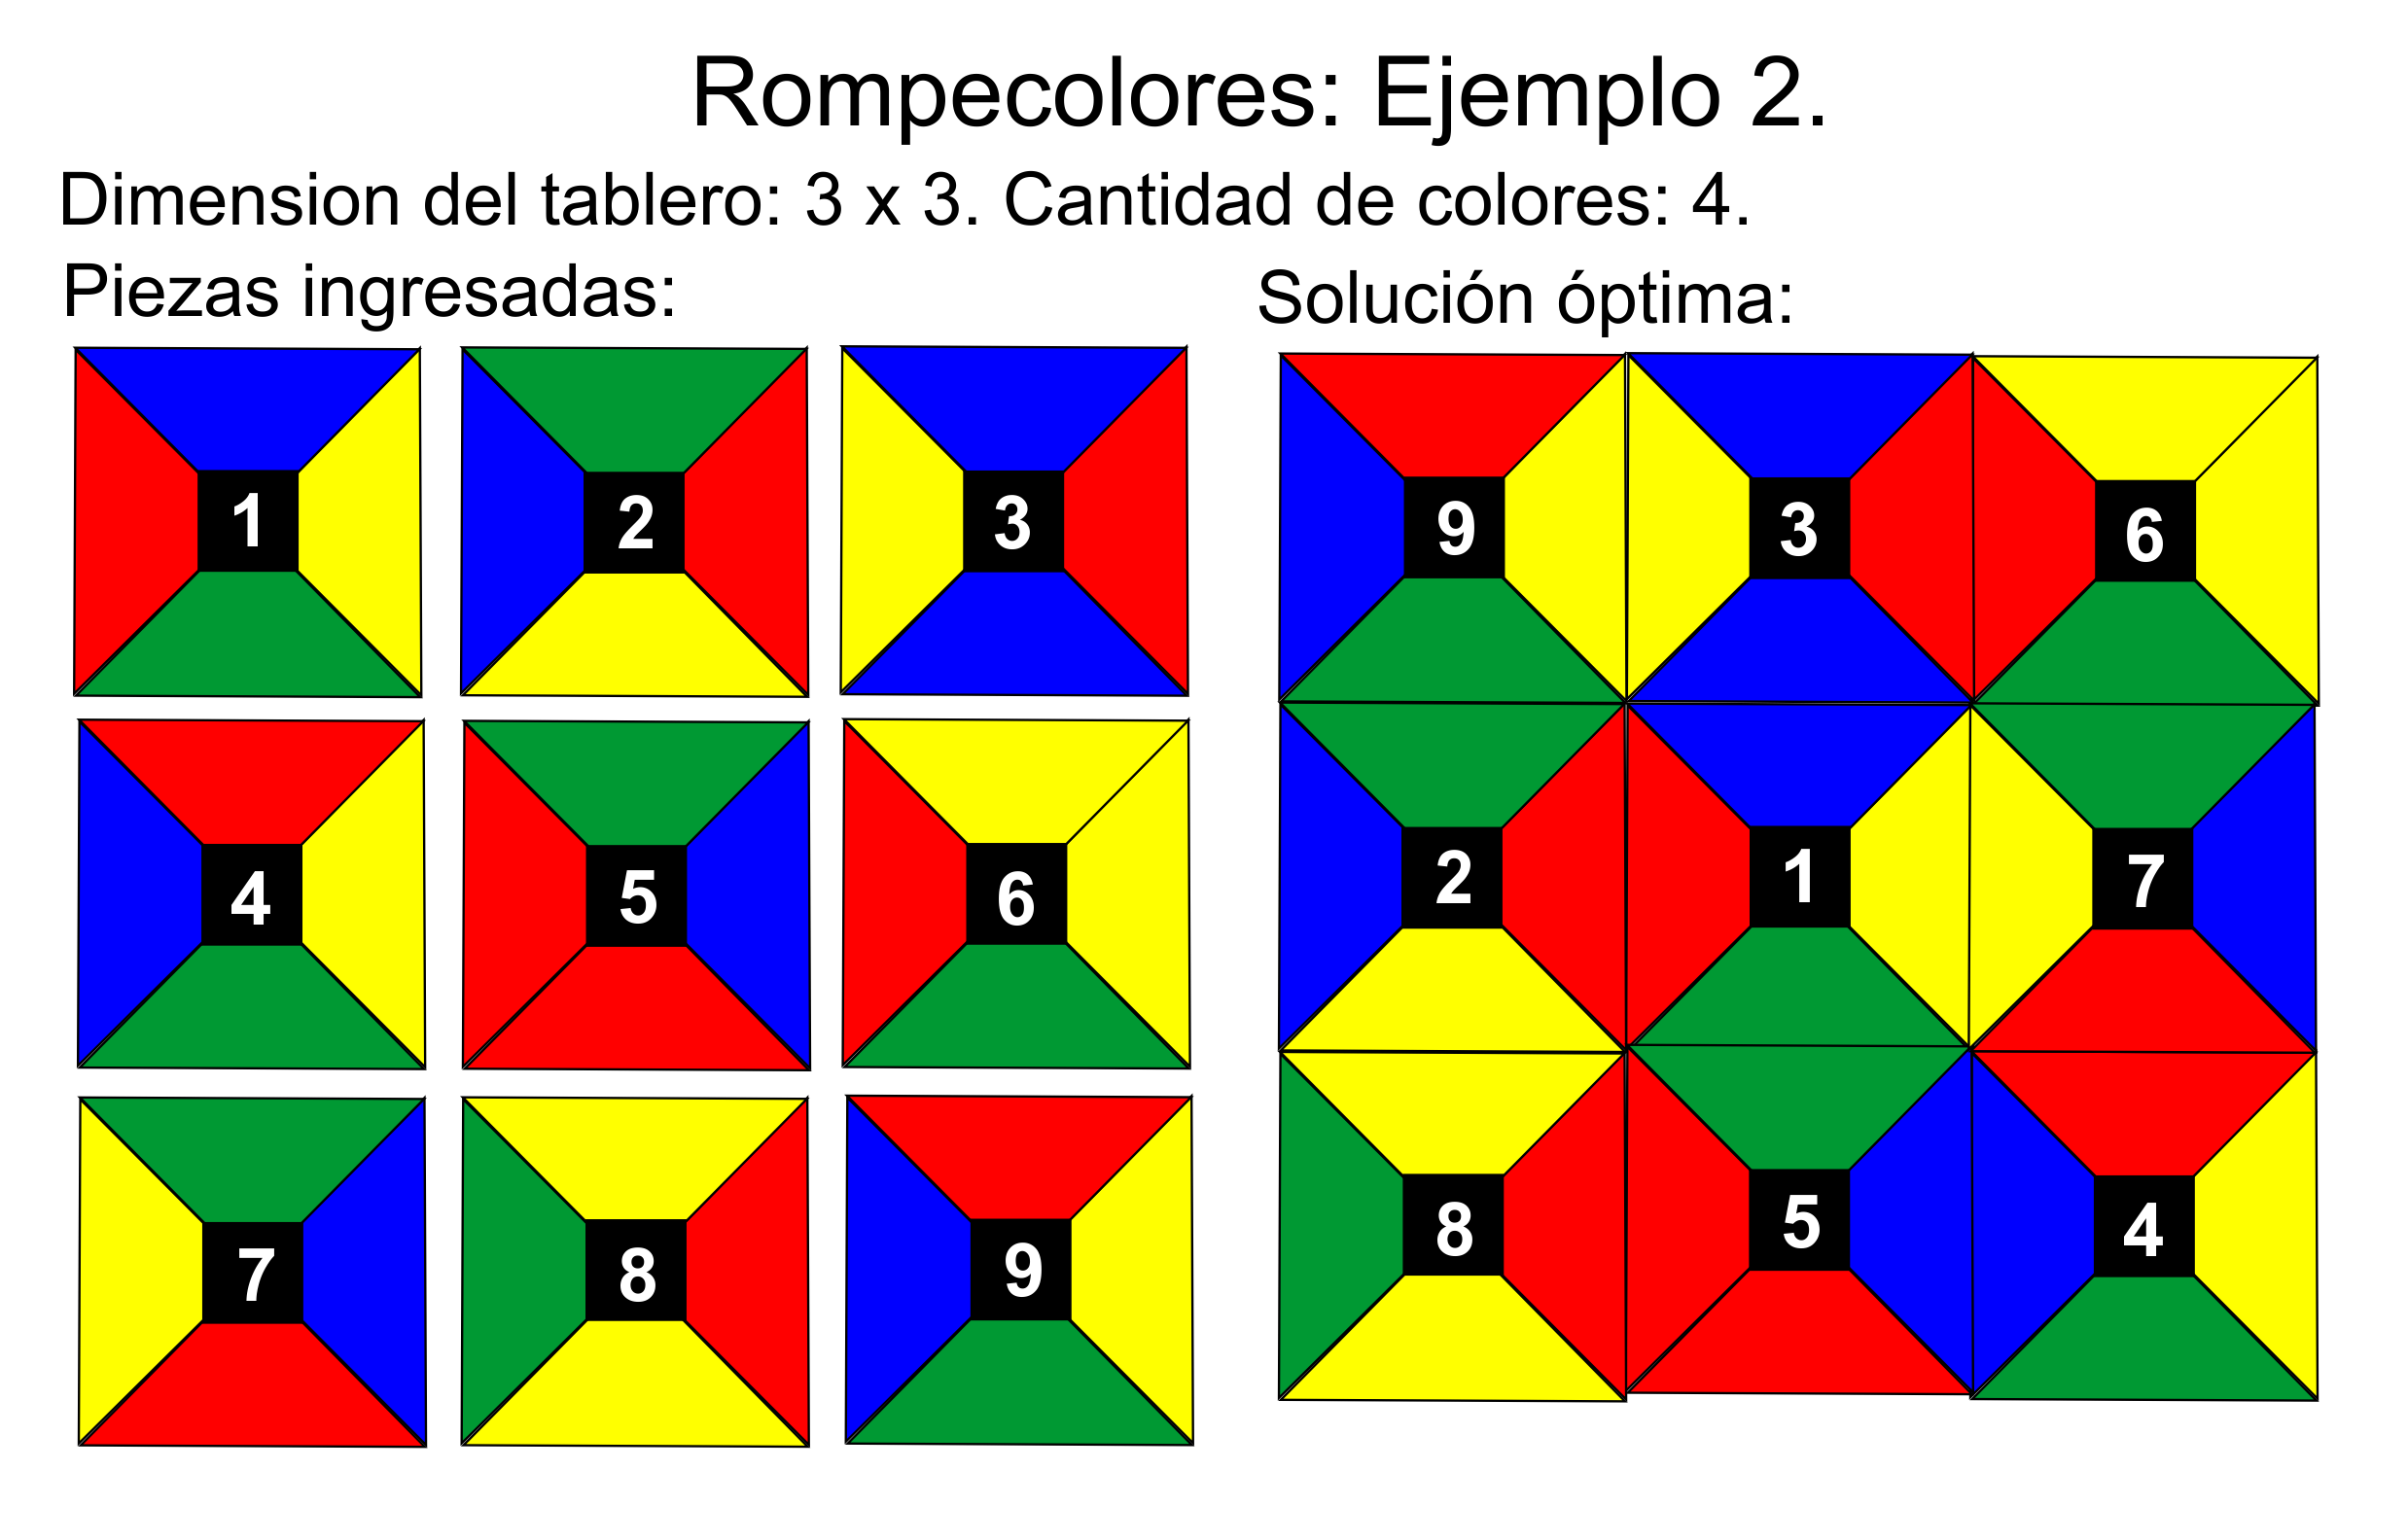
\includegraphics[width=0.6\textwidth]{ejemplo2Compacto}
  \label{fig:ejemplo}
  \caption{Esta es una soluci�n �ptima porque coloca todas las piezas en el tablero.}
\end{figure}



\subsection{Resoluci�n}

Para resolver este problema, lo encaramos de dos maneras distintas, las cuales se pueden ver en \textit{backtracking1.cpp} y \textit{backtracking2.cpp}. El motivo de esto es que, luego de finalizado \textit{backtracking1.cpp}, 
nos dimos cuenta de que era complicado implementar algunas de las podas, especialmente la tercera, por lo cual desarrollamos otra soluci�n, que recorre el espacio de soluciones de otra manera tal que la implementaci�n de dichas podas se facilita. 
Finalmente, cabe se�alar que el primer algoritmo recorre algunos subconjuntos del espacio de soluciones varias veces. Esto implica que con las podas adecuadas el segundo algoritmo puede superarlo. 
En la parte de experimentaci�n, comparamos sus tiempos de ejecuci�n para algunas entradas, ambos teniendo todas las podas activadas.
\newline 
\hspace*{0.5 cm}Las diferencias esenciales entre ambas versiones son que la primera toma una pieza, intenta colocarla en cada posici�n del tablero, y por cada pieza que consigue colocar, recursivamente intenta colocar una segunda pieza en alguna otra posici�n del tablero, etc;
 mientras que la segunda versi�n chequea primero todas las posibles soluciones que surgen de colocar cada una de las $n*m$ piezas en el primer casillero del tablero, luego prueba con el segundo casillero, etc. 
Pero b�sicamente ambas versiones siguen la idea de backtracking, es decir, de explorar sistem�ticamente el espacio de soluciones factibles, siempre que la rama de la recursi�n tenga chances de llegar a una soluci�n �ptima, 
cortando ramas de la recursi�n mediante podas cuando no sea el caso. En el resto del informe, siempre nos referiremos a \textit{backtracking2.cpp}, salvo que explicitemos lo contrario.
\newline
\hspace*{0.5 cm}Las podas que implementamos fueron 4. La primera poda restringe la cantidad de casilleros vac�os que deja la funci�n. 
La segunda poda se fija cu�ntas piezas tengo en mi mejor soluci�n hasta ahora, cu�ntas piezas tengo en mi soluci�n actual, y cu�ntas piezas me quedan por colocar. 
Si la cantidad de piezas en mi mejor soluci�n hasta ahora es mayor o igual que las piezas en mi soluci�n actual m�s la cantidad de piezas restantes, entonces, por m�s que coloque todas las piezas restantes, 
mi soluci�n actual no va a ser mejor que la mejor soluci�n que encontr� hasta ahora; por lo tanto, corto la recursi�n. 
En definitiva, es una poda por altura.
\newline
\hspace*{0.5 cm}La tercera poda consiste en lo siguiente: supongamos que en un nivel k de la recursi�n, colocamos una pieza 'p' en un casillero dado, y exploramos los niveles k+1, k+2, etc., del �rbol recursivo que se genera a partir de esta decisi�n. 
Cuando terminamos de recorrer el �rbol recursivo y volvemos al nivel k de la recursi�n, quitamos la pieza 'p', colocamos en esa posici�n otra pieza 'q', y repetimos el mismo proceso. 
Esta poda se beneficia del hecho de que, si la pieza 'q' es exactamente igual a 'p', es decir, los colores de los 4 bordes coinciden, 
entonces el �rbol de decisiones que se generar�a ser�a id�ntico al de 'p', y por lo tanto estar�amos repitiendo trabajo. 
En este caso, la poda se saltea la pieza 'q' y todas las piezas inmediatamente posteriores que sean iguales a 'p'. 
Para maximizar la efectividad de esta poda, iniciamos el algoritmo con la lista de piezas ordenadas por color, aunque con el paso de las recursiones esta lista puede ir quedando parcial o totalmente desordenada, debido a que va colocando piezas en el tablero, 
y luego en alg�n momento cuando se remueven del tablero, no necesariamente van a quedar en el mismo orden en el que estaban originalmente en la lista de piezas, reduciendo la efectivad de la poda. Una soluci�n a esto ser�a ordenar constantemente la lista de piezas, pero consideramos que esto 
es muy caro e impactar�a negativamente en el tiempo de ejecuci�n final. 

Otra soluci�n posible es armar una estructura de datos que guarde piezas distinguiendo solo por los colores de los lados. Si uno le pide una pieza con el color 1 en todos los lados a esta estructura cuando tiene 2 de ellas, devuelve cualquiera de las dos. Un iterador sobre esta estructura recorrer�a no todas las piezas sino todas las piezas distintas. Lamentablemente, no dispusimos del tiempo para implementar de manera eficiente y correcta una estructura como esta.

Por �ltimo, la cuarta poda chequea si est� en el caso de poder generar una soluci�n trivial. Esto pasar�a si, en un tablero de $n*m$, con una cota de $n*m*4$ posibles colores distintos, los $n*m*4$ colores se encuentran presentes,
lo cual implica necesariamente que todas las piezas tienen colores distintos, y nunca las podr�a colocar juntas. 
Por lo tanto, la �nica soluci�n posible es la trivial, es decir, colocar cada pieza separada de las otras por un casillero en blanco. En la secci�n de correctitud demostramos que generamos la soluci�n de manera tal que es �ptima.
Esta poda es m�s bien una apuesta al todo o nada. 
Si bien ahorra mucho tiempo cuando sirve, no muchas instancias vienen con piezas de colores �nicos. La dejamos porque podemos restringir el costo temporal de verificar la diversidad de colores para solamente entradas con $c=n*m*4$.

\subsection{Correctitud}

\subsubsection{Backtrack sin podas}
Primero vamos a demostrar la correctitud del algoritmo cuando no tiene podas.

\LinesNumbered
\begin{algoritmo}{BacktrackSinPodas}{\Inout{tablero}{Tablero}, \Inout{piezas}{Lista(Pieza)}, \Inout{mejorSolucion}{Lista(PiezaYCoordenada)}, \Inout{solucionPorExplorar}{Lista(PiezaYCoordenada)}, \In{casillero}{Nat}}
	Coordenada posicion \asignar DeterminarCoordenada(casillero, Ancho(tablero))\;
	Nat cantPiezas \asignar Tama�o(piezas)\;
	Nat cantCasillerosRestantes \asignar (Ancho(tablero) * Alto(tablero)) - casillero\;
	\For{\Forcond{i \asignar 1}{cantPiezas}}{
		pieza \asignar PrimeraPieza(piezas)\;
		RemoverPrimerElemento(piezas)\;
		\If{SePuedeInsertarEn(tablero, pieza, posicion)}{
			Insertar(tablero, pieza, posicion)\;
			InsertarAtras(solucionPorExplorar, <pieza, posicion>)\;
			\If{Tama�o(mejorSolucion) < Tama�o(solucionPorExplorar)}{
				mejorSolucion \asignar solucionPorExplorar\;
			}
			\If{casillero < Ancho(tablero) * Alto(tablero) - 1}{
				Backtrack(tablero, piezas, mejorSolucion, solucionPorExplorar, casillero+1)\;
			}
			RemoverPieza(tablero, posicion)\;
			RemoverUltimoElemento(solucionPorExplorar)\;
		}
		InsertarAtras(piezas, pieza)\;
	}
	\If{casillero < Ancho(tablero) * Alto(tablero) - 1}{
		Backtrack(tablero, piezas, mejorSolucion, solucionPorExplorar, casillero+1)\;
	}
\end{algoritmo}

\begin{algoritmo}{DeterminarCoordenada}{\In{casillero}{Nat}, \In{columnas}{Nat}}[Coordenada]
	\return < (casillero / columnas), (casillero $mod$ columnas) >
\end{algoritmo}

\textbf{Tipo Pieza}: Una pieza est� caracterizada por un n�mero identificatorio y cuatro n�meros naturales que representan los colores.

\textbf{Tipo Tablero}: Un tablero est� definido por su ancho, alto, la cantidad de piezas que tiene, y una matriz de piezas.

Algunas de las funciones de tablero son:
\newline
\textit{Ancho()}: Devuelve el ancho del tablero. Coincide con la cantidad de columnas.
\newline
\textit{Alto()}: Devuelve el alto del tablero. Coincide con la cantidad de filas.
\newline
\textit{Insertar(tablero, pieza, pos)}: Coloca 'pieza' en la posici�n 'pos'
\newline
\textit{SePuedeInsertarEn(tablero, pieza, pos)}: Indica si 'pieza' se puede insertar en la posici�n 'pos'. 
Para ello, verifica que el casillero indicado por 'pos' est� vac�o y que los colores inferior, derecho, izquierdo y superior de las piezas circundantes coincidan con los colores superior, izquierdo, derecho e inferior de 'pieza', respectivamente.
\newline
\textit{RemoverPieza(tablero, pos)}: Remueve la pieza ubicada en la posici�n 'pos'.

~\\
Para probar que el algoritmo es correcto, debemos ver que se cumplen 2 cosas:

\begin{enumerate}
 \item Se recorre siempre el espacio entero de soluciones \textbf{factibles}.
 \item Al finalizar el algoritmo, la soluci�n que devuelve es �ptima.
\end{enumerate}

Antes de empezar definimos el espacio total como el conjunto de todos los tableros posibles, teniendo en cuenta que no puede haber una misma pieza (que tenga el mismo n�mero identificador asociado) en dos lugares distintos.
El cardinal de este espacio est� descripto por la funci�n partida $T(p, c)$ donde $p$ es la cantidad de piezas disponibles y $c$ es la cantidad de casilleros que faltan recorrer. Cabe aclarar que $T:\mathbb{N}\times\mathbb{N}\rightarrow \mathbb{N}$.

\[T(p,c) = \left\{
\begin{array}{l l}
  p & \mbox{si c = 1}\\
  p * T(p-1,c-1) + T(p,c-1) & \mbox{en otro caso}\\ 
\end{array} 
\right. 
\]

El cardinal del espacio total para un tablero de $n*m$ ser�a $T(n*m,n*m)$.

~\\
Vamos a probar 1:
\newline
\newline
\-\hspace{0.3cm} El espacio de soluciones \textbf{infactibles} es el subconjunto del espacio total en el cual existe alguna pieza que: 
\begin{itemize}
 \item Su color superior no coincide con el color inferior de la pieza colocada arriba suyo (en el caso en que la pieza no est� en la primera fila)
 \item Su color izquierdo no coincide con el color derecho de la pieza colocada a su izquierda (en el caso en que la pieza no est� en la primera columna)
 \item Su color derecho no coincide con el color izquierdo de la pieza colocada a su derecha (en el caso en que la pieza no est� en la �ltima columna)
 \item Su color inferior no coincide con el color superior de la pieza colocada debajo suyo (en el caso en que la pieza no est� en la �ltima fila)
\end{itemize}

Pero esto nunca puede pasar, ya que solo insertamos una pieza en el tablero cuando SePuedeInsertarEn para esa pieza en esa posici�n da verdadero, y por lo tanto nunca recorremos 
el espacio de soluciones infactibles. Veamos ahora que recorremos el espacio entero de soluciones factibles. 

El algoritmo de backtracking recorre los $n*m$ casilleros a lo largo de las llamadas recursivas. Es decir, la primer llamada mira solamente el primer casillero que lo definimos como el casillero que est� en la esquina superior izquierda. 
El segundo casillero es el que est� a su derecha. Ese es revisado por cualquier llamada a la funci�n Backtrack cuyo valor de casillero sea 1. En cada llamada elige una de las piezas restantes para ese casillero o lo deja vac�o. 

Por ejemplo, si coloca una pieza en el primer casillero entonces va a tener $n*m-1$ piezas para el pr�ximo casillero que mire. En cambio si lo deja vac�o, le quedan todav�a $n*m$.
Esto significa que hay $n*m$ llamadas con $n*m-1$ piezas para el segundo casillero y una llamada con $n*m$ piezas. Vale notar que cada llamada usa una pieza distinta para el primer casillero, si es que se coloca alguna pieza.

En cualquier llamada donde tenemos que hay $p$ piezas restantes y el casillero a mirar es $c$, hay como mucho $T(p,c)$ llamadas recursivas por delante. Aquellas que no se hagan es porque no se pod�a colocar esa pieza en el casillero que estaba mirando.

Finalmente se observa que la primer llamada tiene $n*m$ piezas y $n*m$ casilleros por recorrer.
Con esto vemos que hay a lo sumo $T(n*m,n*m)$ llamadas recursivas. 

El subconjunto del espacio total de soluciones recorrido es el espacio entero de soluciones factibles.
Esto es porque las �nicas disposiciones de tableros descartadas fueron las infactibles por lo dicho al principio.
Por lo tanto, se cumple el punto 1.
~\\
\newline
Veamos que se cumple 2:

Por 1, sabemos que el algoritmo recorre el espacio entero de soluciones factibles. Entre todas ellas se encuentran incluidas las soluciones �ptimas.
Como se puede ver en el pseudoc�digo, cada vez que encuentra una soluci�n parcial cuyo tama�o sea mayor que el de la mejor soluci�n encontrada hasta el momento, la guarda, descartando la anterior. 
Por lo tanto, cuando en alg�n momento de la ejecuci�n llegue a una soluci�n �ptima, que sabemos que va a pasar, necesariamente se va a quedar con esta.



%\begin{verbatim}
% 
% Main():
% 
%    tablero = CrearTablero(n*m)     /* O(n*m) */
%    piezas = CargarPiezas()         /* O(n*m) */
%    mejorSolucion = []                   /* O(1) */
%    solucionPorExplorar = []            /* O(1) */
%    casillero = 0                   /* O(1) */
%    rachaDeSaltos = 0               /* O(1) */
%    
%    Backtrack(tablero, piezas, mejorSolucion, solucionPorExplorar, casillero, rachaDeSaltos)
%    
% end Main
% 
%\end{verbatim}
%\begin{algoritmo}{BacktrackSinPodas}{\Inout{tablero}{Tablero}, \Inout{piezas}{Lista(Pieza)}, \Inout{mejorSolucion}{Lista(PiezaYCoordenada)}, \Inout{solucionPorExplorar}{Lista(PiezaYCoordenada)}, \In{casillero}{Nat}}
%\LinesNumbered
%\nl	Coordenada posicion \asignar DeterminarCoordenada(casillero, Ancho(tablero))\tcc*{$O$(1)}
%	Nat cantPiezas \asignar Tama�o(piezas)\tcc*{$O$(1)}
%	Nat cantCasillerosRestantes \asignar (Ancho(tablero) * Alto(tablero)) - casillero\tcc*{$O$(1)}
%	\tcc{Este ciclo ejecuta $cantPiezas$ veces, que en la primer llamada vale $n*m$}
%	\For(\tcc*[f]{$O$($cantPiezas*Backtrack(casillero+1)$)}){\Forcond{i \asignar 1}{cantPiezas}}{
%		pieza \asignar PrimeraPieza(piezas)\tcc*{$O$(1)}
%		RemoverPrimerElemento(piezas)\tcc*{$O$(1)}
%		\If(\tcc*[f]{$O$(1)}){SePuedeInsertarEn(tablero, pieza, posicion)}{
%			Insertar(tablero, pieza, posicion)\tcc*{$O$(1)}
%			InsertarAtras(solucionPorExplorar, <pieza, posicion>)\tcc*{$O$(1)}
%			\If(\tcc*[f]{$O$(1)}){Tama�o(mejorSolucion) < Tama�o(solucionPorExplorar)}{
%				mejorSolucion = solucionPorExplorar\tcc*{$O$(1)}
%			}
%			\If(\tcc*[f]{$O$(1)}){casillero < Ancho(tablero) * Alto(tablero) - 1}{
%				Backtrack(tablero, piezas, mejorSolucion, solucionPorExplorar, casillero+1) \tcc*{Backtrack($casillero+1$)}
%			}
%			RemoverPieza(tablero, posicion)\tcc*{$O$(1)}
%			RemoverUltimoElemento(solucionPorExplorar)\tcc*{$O$(1)}
%		}
%		InsertarAtras(piezas, pieza)\tcc*{$O$(1)}
%	}
%	\tcc{Esta es la primer poda}
%	\If(\tcc*[f]{$O$(1)}){casillero < Ancho(tablero) * Alto(tablero) - 1}{
%		Backtrack(tablero, piezas, mejorSolucion, solucionPorExplorar, casillero+1) \tcc*{Backtrack($casillero+1$)}
%	}
%\end{algoritmo}

\subsubsection{Backtrack con podas}

A continuaci�n presentamos el algoritmo con podas.

\begin{algoritmo}{Backtrack}{\Inout{tablero}{Tablero}, \Inout{piezas}{Lista(Pieza)}, \Inout{mejorSolucion}{Lista(PiezaYCoordenada)}, \Inout{solucionPorExplorar}{Lista(PiezaYCoordenada)}, \In{casillero}{Nat}, \In{usoPoda1}{\bool}, \In{usoPoda2}{\bool}, \In{usoPoda3}{\bool}, \Inout{usoPoda4}{\bool}}
	Coordenada posicion \asignar DeterminarCoordenada(casillero, Ancho(tablero))\;
	Nat cantPiezas \asignar Tama�o(piezas)\;
	Nat cantCasillerosRestantes \asignar (Ancho(tablero) * Alto(tablero)) - casillero\;
	\tcc{Esta es la cuarta poda}
	\If{CantidadDeColoresMaxima(tablero) == Ancho(tablero)*Altura(tablero)*4  $\land$ usoPoda4}{
		reviso si est�n todos los colores en las piezas\;
		\uIf{est�n todos}{
			GenerarSolucionTrivial(mejorSolucion, piezas, Ancho(tablero), Altura(tablero))\;
		      \return\;
		}\Else{
			usarPoda4 \asignar false\;
		}
	}
	\tcc{Esta es la segunda poda}
	\If{Tama�o(mejorSolucion) $\geq$ Tama�o(solucionPorExplorar) + cantCasillerosRestantes  $\land$ usoPoda2}{
		\return\;
	}
	\For{\Forcond{i \asignar 1}{cantPiezas}}{
		pieza \asignar PrimeraPieza(piezas)\;
		RemoverPrimerElemento(piezas)\;
		\If{SePuedeInsertarEn(tablero, pieza, posicion)}{
			Insertar(tablero, pieza, posicion)\;
			InsertarAtras(solucionPorExplorar, <pieza, posicion>)\;
			\If{Tama�o(mejorSolucion) < Tama�o(solucionPorExplorar)}{
				mejorSolucion \asignar solucionPorExplorar\;
			}
			\If{casillero < Ancho(tablero) * Alto(tablero) - 1}{
				Backtrack(tablero, piezas, mejorSolucion, solucionPorExplorar, casillero+1)\;
			}
			RemoverPieza(tablero, posicion)\;
			RemoverUltimoElemento(solucionPorExplorar)\;
		}
		\tcc{Esta es la tercer poda}
		\While{i < cantPiezas $\land$ usoPoda3}{
			\If{pieza == PrimeraPieza(piezas)}{
				InsertarAtras(piezas, PrimeraPieza(piezas))\;
				RemoverPrimerElemento(piezas)\;
				i++\;
			}
		}
		InsertarAtras(piezas, pieza)\;
	}
	\If{casillero < Ancho(tablero) * Alto(tablero) - 1}{
		\tcc{Esta es la primer poda}
		\If{$\neg$PuedoPonerPiezaEnPosicionPorEncima(tablero, posicionActual) $\lor$ $\neg$usoPoda1}{
			Backtrack(tablero, piezas, mejorSolucion, solucionPorExplorar, casillero+1)\;
		}
	}
\end{algoritmo}

\textit{PuedoPonerPiezaEnPosicionPorEncima}: Indica si puedo poner una pieza cualquiera en la posici�n que est� arriba de la pasada por argumento. Si no existe posici�n por encima, devuelve falso. S�lo devuelve verdadero si existe la posici�n por encima, est� vac�a y los casilleros alrededor suyo tambi�n est�n vac�os (o no existen, si est� en una esquina o borde).


~\\

Para probar que el algoritmo es correcto, debemos ver que se cumplen 3 cosas:
\begin{enumerate}
 \item Se recorre siempre el espacio de soluciones factibles.
 \item Las podas no eliminan soluciones mejores que la obtenida hasta el momento.
 \item Al finalizar el algoritmo, la soluci�n que devuelve es �ptima.
\end{enumerate}

El punto 1 sabemos que se cumple porque vimos que el algoritmo sin podas recorre el espacio entero de las soluciones factibles. Este algoritmo va a evitar explorar algunas ramas de ese subconjunto para tardar menos, pero al igual que el algoritmo anterior, nunca se sale del espacio de soluciones factibles.
\newline
\newline
Ahora veamos que se cumple 2:

La poda 1 corta la recursi�n cuando continuar con ella dejar�a un casillero en blanco que f�cilmente podr�amos rellenar con cualquier pieza. 
Supongamos que estamos en un casillero cualquiera que no sea de la primer fila, $c_0$.
Si podemos insertar una pieza cualquiera en el casillero por encima, entonces cualquier soluci�n que implique saltear este casillero $c_0$, 
la puedo mejorar poniendo una pieza cualquiera en el casillero de la fila anterior y misma columna.\newline\vspace{0.2cm}

Veamos ahora que la poda 2 no elimina soluciones �ptimas: si el tama�o de la mejor soluci�n que encontr� hasta ahora es mayor que el tama�o de la soluci�n que estoy explorando m�s
la cantidad de piezas restantes, entonces por m�s que pudiese colocar todas esas piezas restantes, la mejor soluci�n que encontr� hasta ahora seguir�a siendo mejor que la explorada.
Por lo tanto, no estoy podando ninguna soluci�n �ptima.\newline\vspace{0.2cm}

Veamos ahora que la poda 3 no elimina soluciones �ptimas: esta poda, como se explic� en el punto Resoluci�n, lo �nico que hace es evitar repetir �rboles recursivos.
Por lo tanto, la primera vez que recorro ese �rbol recursivo, si hab�a una soluci�n �ptima, ya la tom�. Evitar recorrer varias veces el mismo �rbol no me imposibilita tomar
la soluci�n �ptima dentro de �l.\newline\vspace{0.2cm}

Veamos finalmente que la poda 4 no elimina soluciones �ptimas: Para que aplique la poda 4, cada uno de los 4 colores de cada una de las $n*m$ piezas debe ser �nico. En ese caso, es imposible que pueda colocar alguna pieza al lado de otra. 
Por lo tanto, una soluci�n �ptima, que es la que terminamos generando, es la trivial, es decir, colocar cada pieza dejando
un casillero vac�o entre cada una. Si se trata de un tablero de cantidad de casilleros par, entonces cualquier tablero generado de esta manera da una soluci�n �ptima porque va a llenar la mitad de los casilleros. 
En cambio, si la cantidad de casilleros es impar, s� importa la forma en que se eligen los casilleros donde se colocan piezas. Esto es porque para una forma de rellenarlo se consiguen colocar $\ceil*{\frac{n*m}{2}}$ y para la otra $\floor*{\frac{n*m}{2}}$.

Entonces con mostrar que generamos la soluci�n que coloca una pieza m�s que la otra para tableros de cantidad de casilleros impares, ya mostramos que es correcta la poda.
Hay s�lo dos formas de elegir los casilleros a rellenar del tablero dejando un casillero entre pieza y pieza. Consideremos un tablero donde los casilleros est�n pintados de blanco y negro como en uno de ajedrez, es decir, al lado de un casillero blanco s�lo hay casilleros negros y viceversa.

El casillero de la esquina superior izquierda (el que adem�s consideramos primero) lo definimos como blanco. Luego el que est� a su derecha, el segundo, es negro. Con esto generamos una partici�n del conjunto de casilleros del tablero con dos clases, negro y blanco.
Entonces es cuesti�n de elegir qu� casilleros llenar: los blancos o los negros. En un tablero de cantidad par de casilleros se puede ver f�cilmente que hay la misma cantidad de casilleros blancos que negros, pero en uno de cantidad impar no.

Consideremos entonces que la cantidad de casilleros es impar. Esto significa que tanto $n$ como $m$ son impares. Miremos primero c�mo es una fila. Empieza con un casillero blanco o negro y termina con un casillero del mismo color por tener una cantidad impar de columnas.
Esto implica que podemos agrupar dos filas contiguas y tendr�amos la misma cantidad de casilleros blancos que de negros. Dicho esto, ignoremos las primeras $n-1$ filas, qued�ndonos con la �ltima nada m�s (suponiendo que $n>1$ si no, aplica igual lo que sigue sin ignorar fila alguna).

Es importante notar que la �ltima fila empieza con un casillero blanco, igual que la primera. Entonces, el �ltimo casillero de la fila tambi�n es blanco. Con esto ya vemos que hay un casillero blanco m�s que casilleros negros.
Dicho r�pidamente: saquemos el primer casillero de esta fila, que es blanco, qued�ndonos con los $m-1$ restantes. Como $m-1$ es par sabemos que ah� tenemos la misma cantidad de casilleros blancos que negros.

Entonces tenemos que la clase blanco tiene un casillero m�s en los tableros de cantidad impar de casilleros que los casilleros negros. Todo lo que queda por hacer es definir esa clase en nuestra matriz de piezas y asegurarnos de que generamos la soluci�n trivial rellenando casilleros de esa clase.

La clase blanco en nuestra matriz est� definida como aquel casillero matriz[$i$][$j$] donde $i$ es el �ndice de fila y vale $0\leq i<n$ y $j$ es el �ndice de columna y vale $0\leq j<m$ que cumple $i+j\quad mod\quad 2 = 0$.
En el c�digo fuente se puede ver que la funci�n generarSolucionTrivial elige los casilleros de esta forma.
\newline
Por lo tanto, se cumple el punto 2.
\newline
\newline
Por �ltimo, 3 se cumple casi por los mismos motivos que en el algoritmo sin podas:

Por 1 y 2, sabemos que el algoritmo recorre el espacio de soluciones factibles y que adem�s, dentro de este espacio de soluciones, est�n las �ptimas.
Como se puede ver en el pseudoc�digo, cada vez que encuentra una soluci�n parcial cuyo tama�o sea mayor que el de la mejor soluci�n que encontr� hasta ahora, me la quedo. 
Por lo tanto, cuando en alg�n momento de la ejecuci�n llegue a una soluci�n �ptima, necesariamente se va a quedar con esta.
\newline
Entonces, por 1, 2 y 3, el algoritmo es correcto.

\subsection{Complejidad}

Para calcular la complejidad de la funci�n Backtrack, definimos la funci�n $T'(p,c)$ en base a la funci�n $T(p,c)$ que usamos para calcular el cardinal del espacio total, que representa el costo temporal que tiene la funci�n con una entrada de $p$ piezas y $c$ casilleros restantes para ver. 

\[T'(p,c) = \left\{
\begin{array}{l l}
  p * union(p) & \mbox{si c = 1}\\
  p * (union(p) + T'(p-1,c-1)) + T'(p,c-1) & \mbox{en otro caso}\\ 
\end{array} 
\right. 
\]


La funci�n $union(p)$ es el costo que tiene la funci�n de backtrack en todas las operaciones que no sean llamadas recursivas. Como se ve en la porci�n de pseudoc�digo a continuaci�n, en el peor caso $union(p) = n*m$ con lo que $union(p) \in O(n*m)$.
~\\
\newline
\begin{algoritmo}{Backtrack}{\Inout{tablero}{Tablero}, \Inout{piezas}{Lista(Pieza)}, \Inout{mejorSolucion}{Lista(PiezaYCoordenada)}, \Inout{solucionPorExplorar}{Lista(PiezaYCoordenada)}, \In{casillero}{Nat}, \In{usoPoda1}{\bool}, \In{usoPoda2}{\bool}, \In{usoPoda3}{\bool}, \Inout{usoPoda4}{\bool}}
	Coordenada posicion \asignar DeterminarCoordenada(casillero, Ancho(tablero))\tcc*{$O$(1)}
	Nat cantPiezas \asignar Tama�o(piezas)\tcc*{$O$(1)}
	Nat cantCasillerosRestantes \asignar (Ancho(tablero) * Alto(tablero)) - casillero\tcc*{$O$(1)}
\end{algoritmo}
\begin{algoritmosimple}
\setcounter{AlgoLine}{16}
	\tcc{Este ciclo ejecuta $cantPiezas$ veces, que en la primer llamada vale $n*m$}
	\For(\tcc*[f]{$O$($cantPiezas*(n*m+T'$($cantPiezas-1$, $(n*m-casillero)-1)$))}){\Forcond{i \asignar 1}{cantPiezas}}{
		pieza \asignar PrimeraPieza(piezas)\tcc*{$O$(1)}
		RemoverPrimerElemento(piezas)\tcc*{$O$(1)}
		\If(\tcc*[f]{$O$(1)}){SePuedeInsertarEn(tablero, pieza, posicion)}{
			Insertar(tablero, pieza, posicion)\tcc*{$O$(1)}
			InsertarAtras(solucionPorExplorar, <pieza, posicion>)\tcc*{$O$(1)}
			\If(\tcc*[f]{$O$(1)}){Tama�o(mejorSolucion) < Tama�o(solucionPorExplorar)}{
				mejorSolucion \asignar solucionPorExplorar\tcc*{$O$($n*m$)}
			}
			\If(\tcc*[f]{$O$(1)}){casillero < Ancho(tablero) * Alto(tablero) - 1}{
				Backtrack(tablero, piezas, mejorSolucion, solucionPorExplorar, casillero+1)\;
				\tcc*{$cantPiezas*T'$($cantPiezas-1$, $(n*m-casillero)-1$)}
			}
			RemoverPieza(tablero, posicion)\tcc*{$O$(1)}
			RemoverUltimoElemento(solucionPorExplorar)\tcc*{$O$(1)}
		}
		\tcc{Esta es la tercer poda}
		\While(\tcc*[f]{$O$($cantPiezas$)}){i < cantPiezas $\land$ usoPoda3}{
			\If(\tcc*[f]{$O$(1)}){pieza == PrimeraPieza(piezas)}{
				InsertarAtras(piezas, PrimeraPieza(piezas))\tcc*{$O$(1)}
				RemoverPrimerElemento(piezas)\tcc*{$O$(1)}
				i++\tcc*{$O$(1)}
			}
		}
		InsertarAtras(piezas, pieza)\tcc*{$O$(1)}
	}
\end{algoritmosimple}
~\\
\newline
Algunas consideraciones adicionales: $cantPiezas \leq n*m \Rightarrow cantPiezas \in O(n*m)$.
Desarrollemos un poco $T'(n*m, n*m)$:

$T'(n*m, n*m) = (n*m) * (n*m + T'(n*m-1, n*m-1)) + T'(n*m, n*m-1) =\\ (n*m)^2 + n*m* T'(n*m-1, n*m-1) + T'(n*m, n*m-1) =\\ (n*m)^2 + n*m* \bigg((n*m-1) * \Big(n*m + T'(n*m-2,n*m-2)\Big) + T'(p,n*m-2)\bigg) + T'(n*m, n*m-1)$

Con esto vemos que emerge un t�rmino $n*m*(n*m)!$ con lo cual el algoritmo tiene complejidad total de $O\big(n*m*(n*m)!\big)$.

El resto de las podas merecen un an�lisis aparte porque evitan iteraciones del algoritmo sin influir mucho en la complejidad asint�tica.
Veamos la complejidad de la cuarta poda:

\begin{algoritmosimple}
\setcounter{AlgoLine}{4}
	\tcc{Esta es la cuarta poda}
	\If(\tcc*[f]{$O$(1)}){CantidadDeColoresMaxima(tablero) = Ancho(tablero)*Altura(tablero)*4  $\land$ usoPoda4}{
		reviso si est�n todos los colores en las piezas\tcc*{$O$($n*m$)}
		\uIf(\tcc*[f]{$O$($n*m$)}){est�n todos}{
			GenerarSolucionTrivial(mejorSolucion, piezas, Ancho(tablero), Altura(tablero))\tcc*{$O$($n*m$)}
		    \return\;
		}\Else{
			usarPoda4 \asignar false\tcc*{$O$(1)}
		}
	}
\end{algoritmosimple}

Como se puede ver, la comparaci�n en la guarda es $O$(1). Esto significa que no influye asint�ticamente una vez que se encuentra desactivada la poda. Si llega a cumplirse la guarda, termina ejecutando el bloque una sola vez. Ejecutar el bloque cuesta $O$($n*m$). Si resulta que est�n todos los $n*m*4$ colores nos ahorramos la complejidad inmensa de $T'(n*m,n*m)$. En caso contrario, pagamos muy poco en relaci�n con lo que va a costar explorar el espacio de soluciones y nos aseguramos de hacerlo solo una vez.

Veamos la complejidad de la segunda poda:

\begin{algoritmosimple}
\setcounter{AlgoLine}{13}
	\tcc{Esta es la segunda poda}
	\If(\tcc*[f]{$O$(1)}){Tama�o(mejorSolucion) $\geq$ Tama�o(solucionPorExplorar) + cantCasillerosRestantes  $\land$ usoPoda2}{
		\return\;
	}
\end{algoritmosimple}

Esta es la mejor poda a nuestra disposici�n. Tiene un costo constante y evita explorar subconjuntos del espacio de soluciones bastante grandes.

Finalmente veamos la complejidad de la primer poda:

\begin{algoritmosimple}
\setcounter{AlgoLine}{40}
	\If(\tcc*[f]{$O$(1)}){casillero < Ancho(tablero) * Alto(tablero) - 1}{
		\tcc{Esta es la primer poda}
		\If(\tcc*[f]{$O$(1)}){$\neg$PuedoPonerPiezaEnPosicionPorEncima(tablero, posicionActual) $\lor$ $\neg$usoPoda1}{
			Backtrack(tablero, piezas, mejorSolucion, solucionPorExplorar, casillero+1)\;
			\tcc*{$T'$($cantPiezas$, $(n*m-casillero)-1$)}
		}
	}
\end{algoritmosimple}

Nuevamente tiene un costo constante como las otras. A priori, su efectividad es cuestionable si est� activada al mismo tiempo que la segunda poda porque ambas apuntan a podar el mismo tipo de soluciones: tableros demasiado vac�os.

\subsection{Testing}

Para hacer el testing consideramos los casos bordes, es decir, cuando todos los colores son iguales, y cuando todos los colores son distintos.

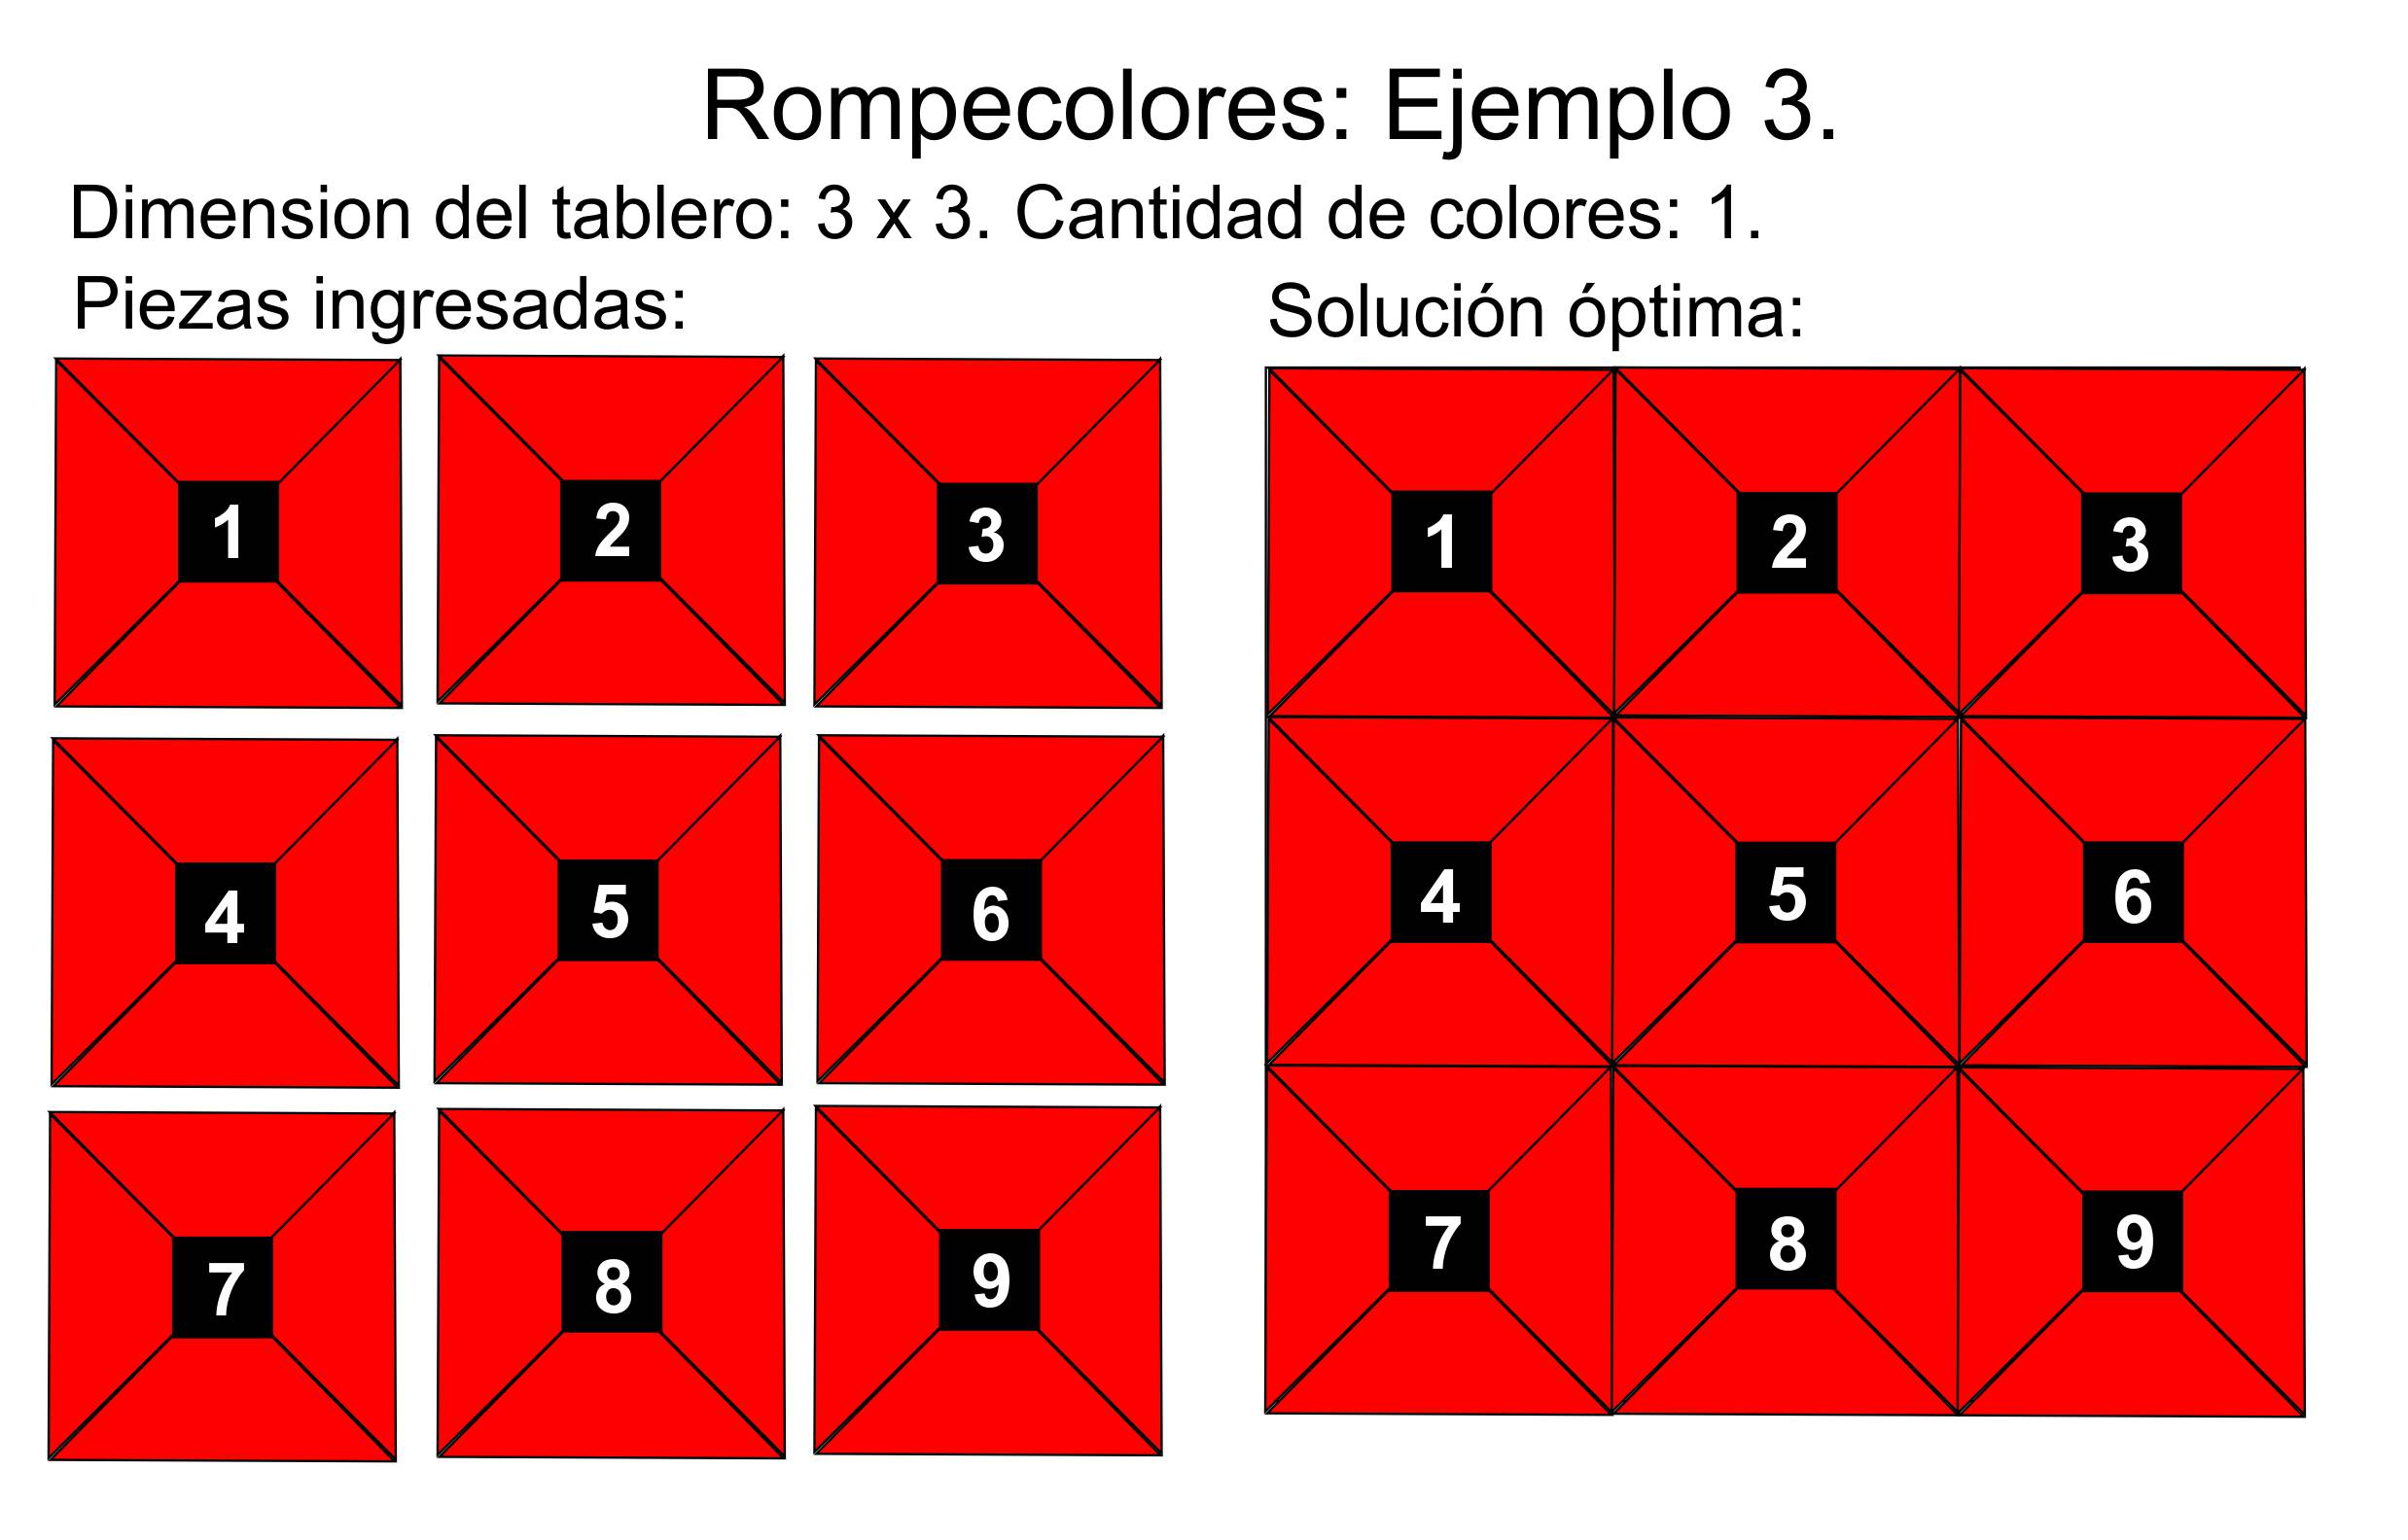
\includegraphics[width = 0.8 \textwidth]{ej3/ejemplo1.jpg}

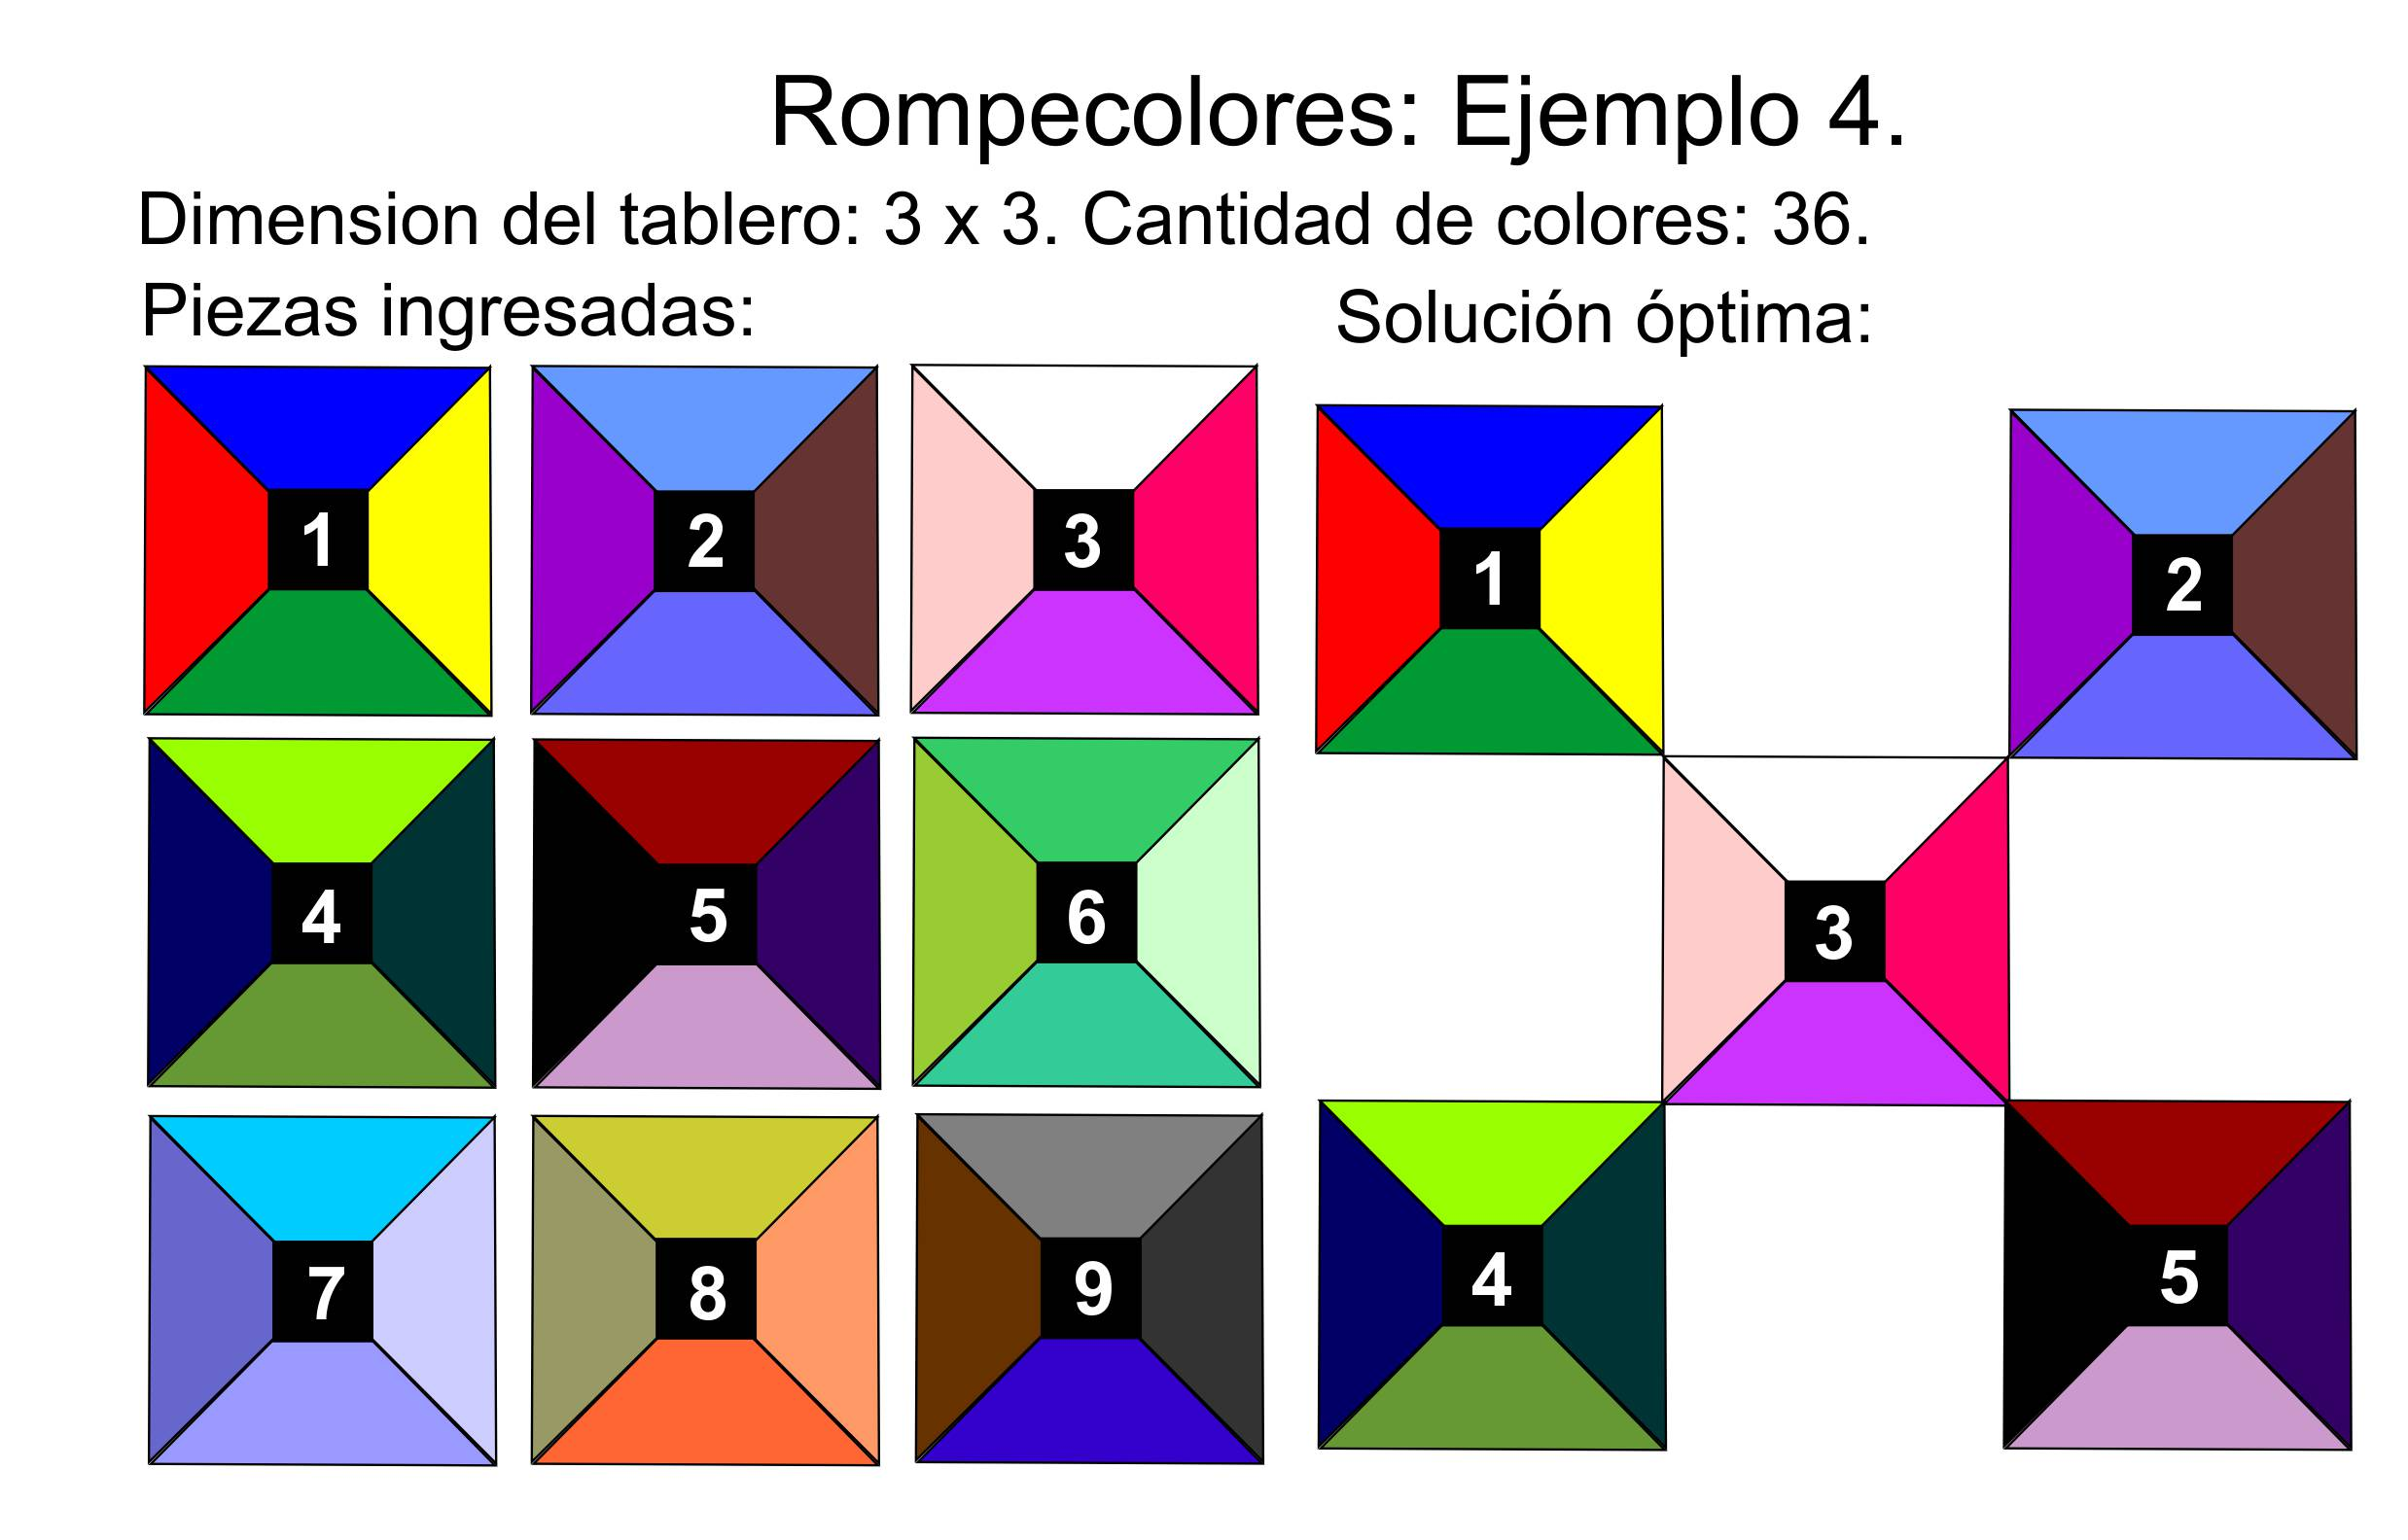
\includegraphics[width = 0.8 \textwidth]{ej3/ejemplo2.jpg}

Como podemos observar, ambas soluciones son las esperadas.




\subsection{Experimentaci�n}

\subsubsection{Generaci�n de Casos Aleatorios}

El generador de casos de test random es genRan y toma exactamente cuatro argumentos.\\
\textbf{genRan targetFile dimensi�n ncolores hilos}\\
El argumento \textbf{targetFile} le da el nombre base del archivo donde va a escribir los tests. Este se escribe en modo 'out' con lo que se destruye
lo que haya en cualquier archivo ya existente con el mismo nombre. El argumento \textbf{hilos}, le indica en cu�ntos archivos repartir los tests generados. 
Si vale 4 por ejemplo, va a generar cuatro archivos: targetFile-1, targetFile-2, targetFile-3 y targetFile-4. 
La idea de esta opci�n es poder ejecutar el backtracking en paralelo sobre una tanda generada.
Los tests que genera son todos los tableros que tienen como m�ximo \textbf{filas*columnas} = \textbf{dimensi�n} casilleros y como mucho \textbf{ncolores} colores.
Para generar los colores de las piezas, utilizamos la funci�n \textbf{rand()} con semilla \textbf{srand(time(NULL))}.

\subsubsection{Instrucciones de uso}

Hay un makefile en el directorio ej3 que corresponde a este problema.
Si se ejecuta make all, va a compilar tanto el backtrack1 como el backtrack2, y adem�s el generador de tests random.
El backtrack1 es el algoritmo que recorre de manera no �nica el espacio de soluciones intentando poner todas las piezas que puede.
El backtrack2 es el algoritmo que analizamos y podamos lo m�s posible dado que s� recorr�a de manera �nica el espacio de posibilidades.
Si no se desean tomar mediciones, la manera de ejecutarlo es la normal, redireccionando el archivo que contiene las instancias de test. Ej: ./backtrack2 < instanciasTest.
~\\
\\
En caso de querer tomar mediciones, se deben especificar los siguientes par�metros adicionales: un primer par�metro con el nombre del archivo en donde se desean guardar las mediciones, y 
un segundo, tercer y cuarto par�metro, correspondientes a las podas 1, 2 y 3 respectivamente, que deber�n ser \textbf{1} para activar la poda y \textbf{0} para desactivarla. Luego se deber� 
redireccionar el archivo que contiene las instancias de test. Ej: ./backtrack2 archivoMediciones 1 1 1 < instanciasTest, en donde se est�n activando las 3 podas y guardando los resultados de las
 mediciones en ``archivoMediciones''.



\subsubsection{Resultados}

Primero presentamos un gr�fico que compara el backtrack1 contra el 2. A continuaci�n se ven gr�ficos para tableros $n$ filas, $m$ columnas y $n*m$ colores con distintas podas activadas.
Finalmente hay gr�ficos para tableros de $n*m*4$ colores, nuevamente con distintas podas activadas.
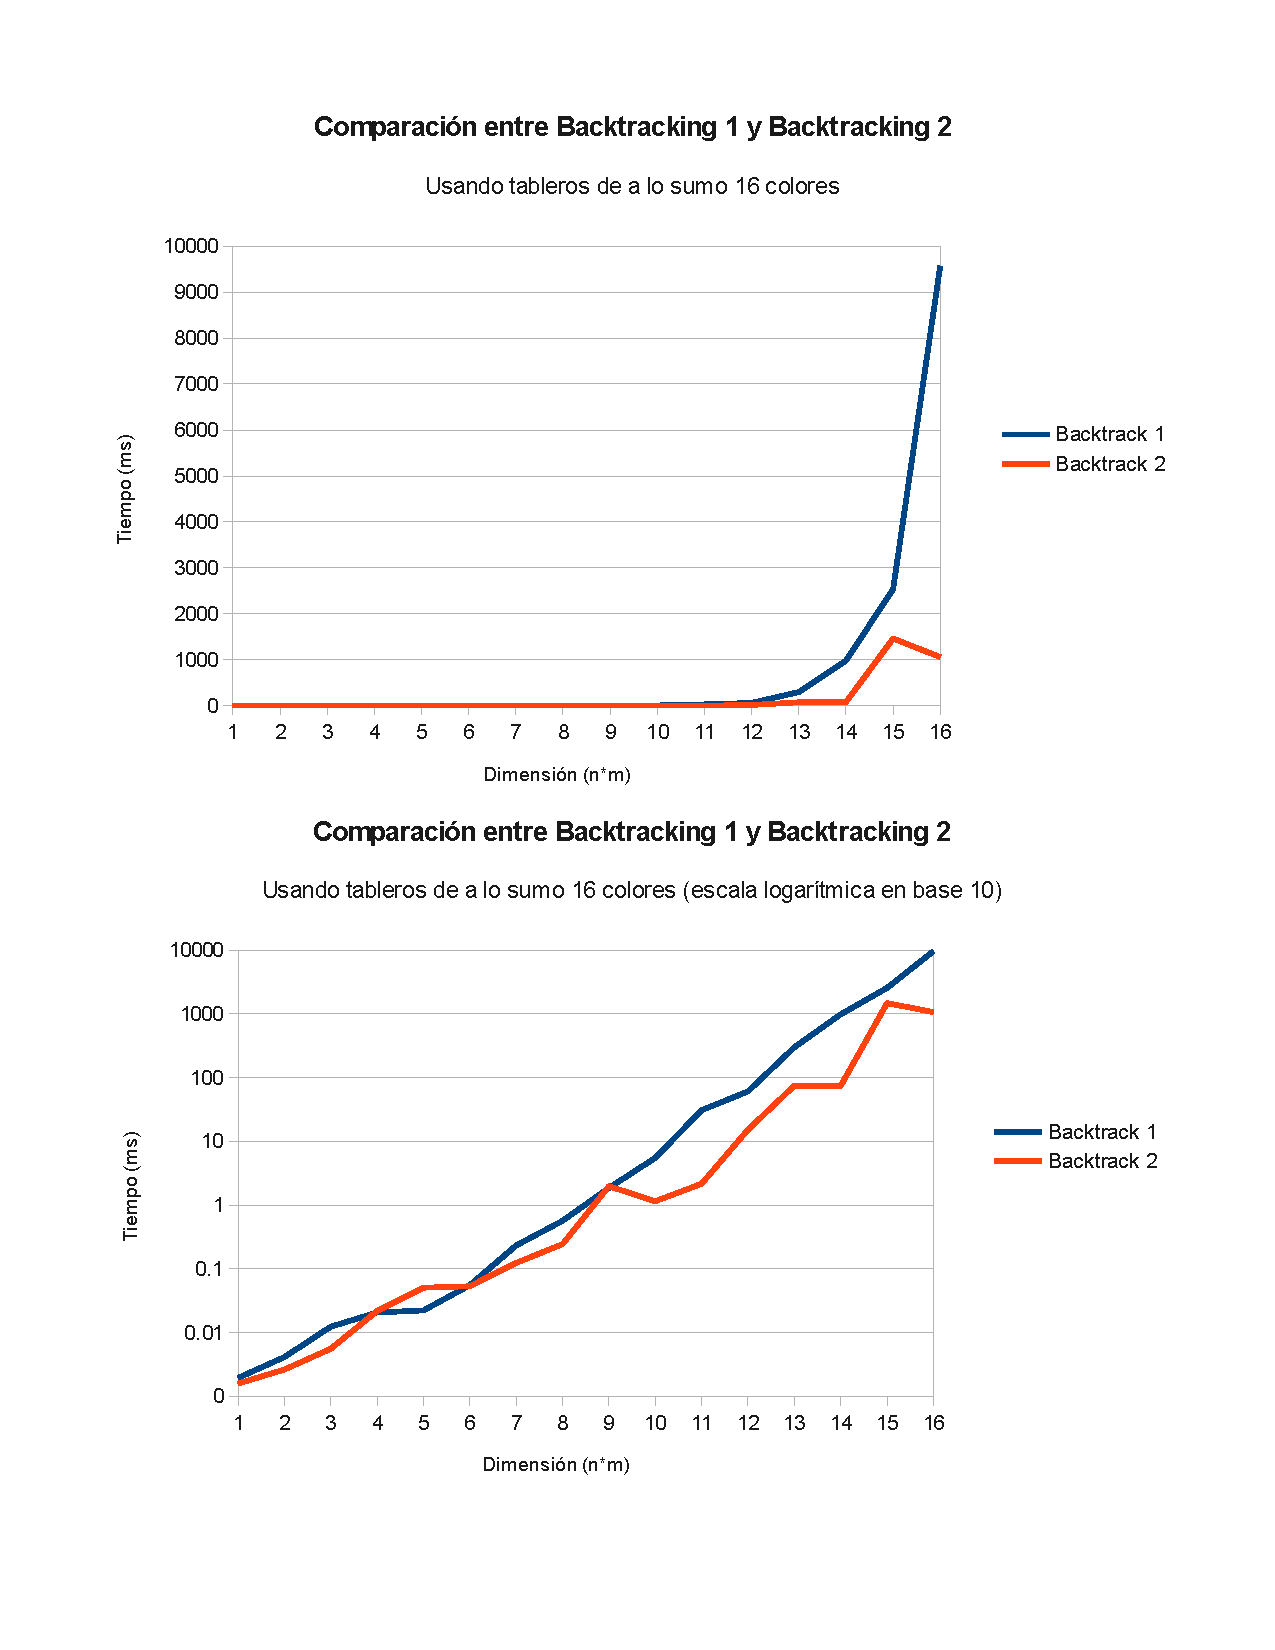
\includepdf[pages={1}]{ej3/mediciones/comparacion/comparacion_nueva.pdf}
\includepdf[pages={1}]{ej3/mediciones/1color/graficos_nuevos.pdf}
\includepdf[pages={1}]{ej3/mediciones/10colores/graficos_nuevos.pdf}
\includepdf[pages={1}]{ej3/mediciones/n*m/graficos_nuevos.pdf}
\includepdf[pages={1}]{ej3/mediciones/n*m*4/graficos_nuevos.pdf}


\subsubsection{Conclusiones}

Las conclusiones que pudimos sacar en cuanto a las 2 versiones de backtracking fue lo que esperabamos: la versi�n 2 es claramente m�s r�pida que la versi�n 1.
En cuanto a las podas, pudimos ver una tendencia que se mantuvo para distintas cantidades de colores: la poda 1 se mostr� totalmente inefectiva, superando en algunos casos a la versi�n sin podas en tiempo de ejecuci�n.
La poda 2 resulto ser la m�s efectiva, siendo la que siempre tomaba el menor tiempo de ejecuci�n, seguida de la poda 3, que funciono bien para tableros chicos, pero a partir de $n*m = 10$ aproximadamente, comenz� 
a mostrarse ineficiente.

\subsection{Desarrollo de los ejercicios adicionales}

\subsubsection{Modificaci�n del algoritmo}
Para hacer que el algoritmo funcione en un tablero toroidal basta con modificar la funci�n SePuedeInsertarEn para que revise los casilleros del otro extremo de la matriz cuando est� en un borde.
\subsubsection{Impacto en las podas desarrolladas}
La cuarta poda, donde se revisa si se tienen $n*m*4$ colores en las piezas ya no es correcta. El problema es que la generaci�n de la soluci�n trivial asume que se trata de un tablero con bordes y esquinas, no uno donde todo casillero tiene cuatro vecinos. Si se adapta la generaci�n de la soluci�n trivial al tablero toroidal se puede seguir usando.

La primer poda sigue funcionando y tiene un efecto interesante. Como el casillero que est� por encima del primero est� vac�o y tambi�n los contiguos sin incluir al primero, nunca podr�a dejar vac�o un casillero en la primera llamada. Es probable que esta poda sea m�s efectiva en este tablero toroidal que en el rectangular.

Las otras dos podas no se ven afectadas por la forma del tablero, ya que una es una poda por altura, y la otra una poda que evita repetir �rboles recursivos, y ambas cosas son independientes de la forma del tablero.
\subsubsection{Poda para un tablero toroidal}
La mejor poda que se nos ocurri� consiste en explorar cada disposici�n relativa de piezas una sola vez. Con esto se quiere decir que, por ejemplo, si ya se prob� en alg�n momento colocar la pieza 1 en el primer casillero y la pieza 2 dos casilleros a la derecha del primero, entonces no tiene sentido probar la pieza 1 en el casillero k y la pieza 2 nuevamente dos casilleros su derecha.



\end{document}
